\documentclass[10pt,aspectratio=169]{beamer}

% ── Idioma y fonts ────────────────────────────────────────────────────────────
\usepackage[utf8]{inputenc}
\usepackage[T1]{fontenc}
\usepackage[spanish]{babel}
\usepackage{lmodern}
\usepackage{helvet}
\renewcommand{\familydefault}{\sfdefault}
% Texto en Helvetica sans, pero math con fuentes lmodern correctas:
% evita que beamer sustituya las fuentes math (las griegas mayúsculas
% \Delta,\Theta,\Phi salían como cuadros negros en T1 sans).
\usefonttheme{professionalfonts}

% ── Tema ──────────────────────────────────────────────────────────────────────
\usetheme{Madrid}
\usecolortheme{default}

% Paleta personalizada (azul PUCP-like)
\definecolor{pucpblue}{RGB}{27, 65, 119}
\definecolor{pucpaccent}{RGB}{200, 16, 46}
\definecolor{lightgrey}{RGB}{240, 240, 240}

\setbeamercolor{structure}{fg=pucpblue}
\setbeamercolor{title}{fg=white,bg=pucpblue}
\setbeamercolor{frametitle}{fg=white,bg=pucpblue}
\setbeamercolor{block title}{fg=white,bg=pucpblue}
\setbeamercolor{block body}{bg=lightgrey}
\setbeamercolor{alerted text}{fg=pucpaccent}
\setbeamercolor{section in head/foot}{fg=white,bg=pucpblue}
\setbeamercolor{subsection in head/foot}{fg=white,bg=pucpblue!80}
\setbeamercolor{author in head/foot}{fg=white,bg=pucpblue}
\setbeamercolor{title in head/foot}{fg=white,bg=pucpblue!90}
\setbeamercolor{date in head/foot}{fg=white,bg=pucpblue!80}

\setbeamertemplate{navigation symbols}{}
\setbeamertemplate{caption}[numbered]
\setbeamerfont{caption}{size=\scriptsize}
\setbeamerfont{frametitle}{series=\bfseries,size=\large}

% ── Slides divisores automáticos al inicio de cada sección ───────────────────
\AtBeginSection[]{%
  {%
  \setbeamercolor{background canvas}{bg=pucpblue}
  \setbeamertemplate{headline}{}
  \setbeamertemplate{footline}{}
  \begin{frame}[plain]
  \vfill
  \centering
  \color{white}
  {\Huge\bfseries \insertsectionhead}\par
  \vfill
  \end{frame}
  }%
}

% ── Paquetes ──────────────────────────────────────────────────────────────────
\usepackage{graphicx}
\graphicspath{{output/figures/}}
\usepackage{amsmath,amssymb}
\usepackage{booktabs}
\usepackage{multirow}
\usepackage{array}
\usepackage{caption}
\usepackage{tikz}
\usepackage{xcolor}
\usepackage{hyperref}

% Colores para marcar los supuestos del modelo (Apéndice B)
\definecolor{verdeverdicto}{RGB}{0, 110, 60}
\definecolor{naranjasupp}{RGB}{160, 60, 0}

% Fix babel-spanish: `\,\%` (thin space + porcentaje) en modo math dispara
% \es@sppercent y rompe con "Incompatible glue units". Se restaura `\%` plano.
\AtBeginDocument{\def\%{\char`\%\relax}}

% ── Datos ─────────────────────────────────────────────────────────────────────
\title[Impacto ChatGPT en GitHub]{Impacto de la disponibilidad de ChatGPT en el desarrollo de software orientado a Ciencia de Datos (2020--2023)}
\subtitle{Sustentación de tesis para optar al título de Licenciado en Economía}
\author[Nicho \& Janampa]{Jesus Alberto Nicho Rosado \\ Karl Willem Janampa Aparicio}
\institute[PUCP]{Pontificia Universidad Católica del Perú \\ Facultad de Ciencias Sociales \\[0.3em] {\small Asesor: Alexander Wilder Quispe Rojas}}
\date{Lima, 2026}

\begin{document}

% ════════════════════════════════════════════════════════════════════════════
% PORTADA
% ════════════════════════════════════════════════════════════════════════════
{
\setbeamertemplate{headline}{}
\setbeamertemplate{footline}{}
\begin{frame}[plain]
\titlepage
\end{frame}
}

% ════════════════════════════════════════════════════════════════════════════
% AGENDA
% ════════════════════════════════════════════════════════════════════════════
\begin{frame}{Agenda de la sustentación}
\vspace{0.5em}
\begin{columns}[T]
\begin{column}{0.5\textwidth}
\begin{enumerate}
  \item[\textbf{1.}] Motivación y problemática
  \item[\textbf{2.}] Pregunta e hipótesis
  \item[\textbf{3.}] Marco teórico
  \item[\textbf{4.}] Evidencia empírica previa
  \item[\textbf{5.}] Línea de tiempo de ChatGPT
\end{enumerate}
\end{column}
\begin{column}{0.5\textwidth}
\begin{enumerate}
  \item[\textbf{6.}] Datos y diseño del panel
  \item[\textbf{7.}] Metodología (DiD, CS, SDiD)
  \item[\textbf{8.}] Resultados principales
  \item[\textbf{9.}] Pruebas de robustez
  \item[\textbf{10.}] Limitaciones y conclusiones
\end{enumerate}
\end{column}
\end{columns}
\end{frame}

% ════════════════════════════════════════════════════════════════════════════
\section{1. Motivación}
% ════════════════════════════════════════════════════════════════════════════

\begin{frame}{Motivación}
\begin{itemize}
  \item ChatGPT (OpenAI, 30 noviembre 2022) marcó un punto de inflexión en la asistencia con IA generativa para tareas de programación.
  \item Su escala fue cualitativamente distinta a tecnologías previas (Copilot, Codex): \alert{servicio gratuito, masivo y conversacional}.
  \item Su \alert{disponibilidad geográfica heterogénea} ---bloqueado en China, Rusia, Irán, Cuba, Corea del Norte, entre otros--- generó un escenario cuasi-experimental natural.
  \item El sector software se proyectaba a USD 600\,000 millones para 2025 (Statista, 2023). Toda mejora marginal en productividad tiene consecuencias agregadas relevantes.
\end{itemize}
\end{frame}

\begin{frame}{¿Por qué importa?}
\begin{block}{La pregunta práctica}
Si ChatGPT efectivamente aumenta la productividad o la entrada de desarrolladores, sus implicaciones cruzan tres dimensiones:
\end{block}

\begin{columns}[T]
\begin{column}{0.32\textwidth}
\textbf{\textcolor{pucpblue}{Política pública}}
\medskip

\small Subsidios al acceso, regulación de servicios IA, restricciones internacionales.
\end{column}
\begin{column}{0.32\textwidth}
\textbf{\textcolor{pucpblue}{Empresas}}
\medskip

\small Inversión en suscripciones premium, programas de adopción, evaluación de productividad.
\end{column}
\begin{column}{0.32\textwidth}
\textbf{\textcolor{pucpblue}{Educación}}
\medskip

\small Currículos de ciencia de datos, formación de juniors, certificaciones laborales.
\end{column}
\end{columns}

\vspace{1em}
\centering \alert{Sin evidencia causal robusta, las decisiones se toman a ciegas.}
\end{frame}

% ════════════════════════════════════════════════════════════════════════════
\section{2. Pregunta e hipótesis}
% ════════════════════════════════════════════════════════════════════════════

\begin{frame}{Pregunta de investigación}
\vfill
\begin{block}{Pregunta central}
\centering
¿La \textbf{disponibilidad de ChatGPT} causó un incremento del número de desarrolladores activos en GitHub en los países con acceso, comparado con los países donde el servicio fue restringido, entre 2020 y 2023?
\end{block}

\vfill
\textbf{Unidad de análisis:} país $\times$ lenguaje de programación $\times$ trimestre.

\textbf{Tratamiento:} acceso público a ChatGPT a partir de noviembre 2022.

\textbf{Variable de resultado:} \textit{unique pushers} por cada 100\,000 habitantes.

\textbf{Período:} Q1-2020 a Q4-2023 (16 trimestres).
\vfill
\end{frame}

\begin{frame}{Hipótesis}
\begin{itemize}
  \item \textbf{H1.} La accesibilidad a ChatGPT se asocia positivamente con el desarrollo de software en los países tratados.
  \item \textbf{H2.} El efecto es \alert{heterogéneo por lenguaje}: más fuerte en Python y JavaScript dada su vasta documentación técnica disponible en internet, recurso fundamental para el entrenamiento del modelo.
\end{itemize}

\vspace{1em}
\begin{block}{Mecanismos teóricos detrás de las hipótesis}
\begin{enumerate}
  \item \textbf{Reasignación de tareas} (Acemoglu \& Restrepo, 2018, 2019): la IA libera tareas rutinarias, expande la frontera de proyectos rentables y atrae programadores marginales.
  \item \textbf{Reducción de costos de búsqueda y aprendizaje} (Stigler, 1961): ChatGPT colapsa el costo de explorar documentación y foros a niveles cercanos a cero.
\end{enumerate}
\end{block}
\end{frame}

% ════════════════════════════════════════════════════════════════════════════
\section{3. Marco teórico}
% ════════════════════════════════════════════════════════════════════════════

\begin{frame}{Marco teórico (I): Acemoglu \& Restrepo}
\begin{block}{Tecnología como reasignador de tareas}
El cambio tecnológico actúa en dos canales simultáneos sobre el trabajo:
\end{block}

\begin{columns}[T]
\begin{column}{0.48\textwidth}
\textbf{\textcolor{pucpaccent}{Displacement effect}}
\medskip

\small ChatGPT automatiza tareas previamente del programador:
\begin{itemize}\small
  \item Búsqueda de sintaxis
  \item Redacción de \textit{boilerplate}
  \item Depuración rutinaria
\end{itemize}
\end{column}
\begin{column}{0.48\textwidth}
\textbf{\textcolor{pucpblue}{Reinstatement effect}}
\medskip

\small Al bajar el costo marginal de producir código:
\begin{itemize}\small
  \item Proyectos antes inviables se vuelven rentables.
  \item Programadores marginales pueden entrar.
  \item La frontera productiva se expande.
\end{itemize}
\end{column}
\end{columns}

\vspace{1em}
\centering \alert{Efecto neto sobre la actividad de desarrollo: positivo bajo condiciones plausibles.}
\end{frame}

\begin{frame}{Marco teórico (II): Stigler y la economía de la información}
\begin{block}{Costos de búsqueda y de aprendizaje}
Stigler (1961) modela la búsqueda como un costo que el agente paga para reducir incertidumbre sobre alternativas.
\end{block}

\textbf{En desarrollo de software, este costo se traduce en:}
\begin{itemize}
  \item Tiempo dedicado a leer documentación oficial.
  \item Búsquedas en Stack Overflow, foros, tutoriales.
  \item Experimentación con código que falla.
\end{itemize}

\vspace{0.5em}
\textbf{ChatGPT actúa como un \textit{shock} negativo sobre estos costos:} ofrece respuestas contextualizadas e instantáneas.

\vspace{0.5em}
\begin{exampleblock}{Evidencia coherente: Del Río-Chanona et al.\ (2023)}
\textbf{$-16\,\%$} en actividad de Stack Overflow tras el lanzamiento de ChatGPT $\Rightarrow$ reorganización endógena de los canales de búsqueda.
\end{exampleblock}
\end{frame}

\begin{frame}{Marco teórico (III): modelo formal de adopción heterogénea}
\small
\begin{block}{De la tarea individual al panel agregado}
El desarrollador elige el método más productivo en cada tarea $z\in[0,1]$:
\[
y_{jc}(z;\mu_j)=\max\{h_c(z),\,\mu_j\,a_c(z)\},\qquad \mu_j\in\{0,1\}.
\]
\end{block}

\begin{columns}[T]
\begin{column}{0.5\textwidth}
\centering\textbf{\textcolor{pucpblue}{Exposición del lenguaje}}
\[
\theta_c=\underbrace{\tau_c}_{\substack{\text{frac.\ tareas}\\\text{automatizables}}}\!\cdot\!\underbrace{\rho_c}_{\substack{\text{ahorro}\\\text{relativo}}}
\]
\end{column}
\begin{column}{0.5\textwidth}
\centering\textbf{\textcolor{pucpblue}{Absorción del país}}
\[
\phi_i=10^5\,f_i\!\bigl(\eta^*_c(0)\bigr)
\]
\end{column}
\end{columns}

\vspace{0.4em}
\begin{exampleblock}{Ecuación estimable (resultado del modelo)}
\centering
$Y_{ict}=\alpha_i+\beta_t+\delta_c+\textcolor{pucpaccent}{\theta_c\,\phi_i}\,A_{it}+\eta_{ict}$
\end{exampleblock}
\centering\footnotesize El coeficiente del tratamiento se factoriza en \textbf{exposición} ($\theta_c$, por lenguaje) y \textbf{absorción} ($\phi_i$, por país) $\Rightarrow$ sustenta la \textbf{H2}. \textit{Derivación completa de 8 pasos en el Apéndice~B.}
\end{frame}

% ════════════════════════════════════════════════════════════════════════════
\section{4. Evidencia empírica}
% ════════════════════════════════════════════════════════════════════════════

\begin{frame}{Evidencia empírica: impacto económico de la IA}
\vspace{0.2em}
\renewcommand{\arraystretch}{1.30}
\centering
\footnotesize
\begin{tabular}{p{3.5cm}p{2.2cm}p{8cm}}
\toprule
\textbf{Autor} & \textbf{Efecto} & \textbf{Resultado breve} \\
\midrule
Brynjolfsson et al.\ (2023) & \textcolor{green!45!black}{$\uparrow$ \textbf{Positivo}} & $\uparrow$ $14\,\%$ la productividad en atención al cliente, especialmente en empleados con menor experiencia. \\
Gallea (2023) & \textcolor{green!45!black}{$\uparrow$ \textbf{Positivo}} & $\downarrow$ preguntas comunes en Stack Overflow y orienta a los usuarios hacia consultas más complejas. \\
Wu et al.\ (2024) & \textcolor{green!45!black}{$\uparrow$ \textbf{Positivo}} & $\uparrow$ valor de mercado de las empresas chinas que decidieron integrar la IA. \\
Liu et al.\ (2023) & \textcolor{orange!75!black}{$\approx$ \textbf{Neutro}} & $\downarrow$ la demanda de trabajos automatizables, pero favoreció a freelancers que lo integraron en su servicio. \\
Del Río-Chanona et al.\ (2023) & \textcolor{pucpaccent}{$\downarrow$ \textbf{Negativo}} & $\downarrow$ uso de foros como Stack Overflow, afectando la generación de datos públicos para entrenar IA. \\
Demirci et al.\ (2023) & \textcolor{pucpaccent}{$\downarrow$ \textbf{Negativo}} & $\downarrow$ demanda de tareas automatizables y de generación de imágenes. \\
Hui et al.\ (2023) & \textcolor{pucpaccent}{$\downarrow$ \textbf{Negativo}} & $\downarrow$ el empleo y los ingresos de \textit{freelancers} en ocupaciones vulnerables como redacción y edición. \\
\bottomrule
\end{tabular}
\end{frame}

\begin{frame}{Evidencia empírica: capacidades por lenguaje de programación}
\vspace{0.3em}
\renewcommand{\arraystretch}{1.35}
\centering
\footnotesize
\begin{tabular}{p{3.5cm}p{2.2cm}p{8cm}}
\toprule
\textbf{Autor} & \textbf{Efecto} & \textbf{Resultado breve} \\
\midrule
Buscemi (2023) & \textcolor{green!45!black}{$\uparrow$ \textbf{Positivo}} & En ciencia de datos, Julia mostró el mejor desempeño ($81{,}5\,\%$), seguido de R y Python, destacando la eficacia del modelo en lenguajes populares y especializados en análisis estadístico. \\
Chai et al.\ (2024) & \textcolor{green!45!black}{$\uparrow$ \textbf{Positivo}} & Usando el \textit{benchmark} MCEVAL, se evidenció que el rendimiento de ChatGPT-3.5 Turbo varía ampliamente entre lenguajes: destaca en Python, Java y Ruby, pero muestra limitaciones en lenguajes menos comunes como Elisp, Scheme y VimL. \\
Li y Krishnamachari (2024) & \textcolor{green!45!black}{$\uparrow$ \textbf{Positivo}} & MultiPL-LeetCode mostró que el rendimiento de ChatGPT-3.5 Turbo varía según el lenguaje: es alto en Python, Java y C++, pero deficiente en lenguajes funcionales como Elixir, Erlang y Racket. \\
\bottomrule
\end{tabular}

\vspace{0.6em}
\begin{block}{Brecha en la literatura}
\centering \footnotesize Ningún estudio analiza específicamente el impacto causal de ChatGPT sobre el \textbf{desarrollo de software} desagregado por lenguaje a nivel de país.
\end{block}
\end{frame}

% ════════════════════════════════════════════════════════════════════════════
\section{5. Línea de tiempo}
% ════════════════════════════════════════════════════════════════════════════

\begin{frame}{Línea de tiempo: ChatGPT y limitaciones (2020--2023)}
\centering
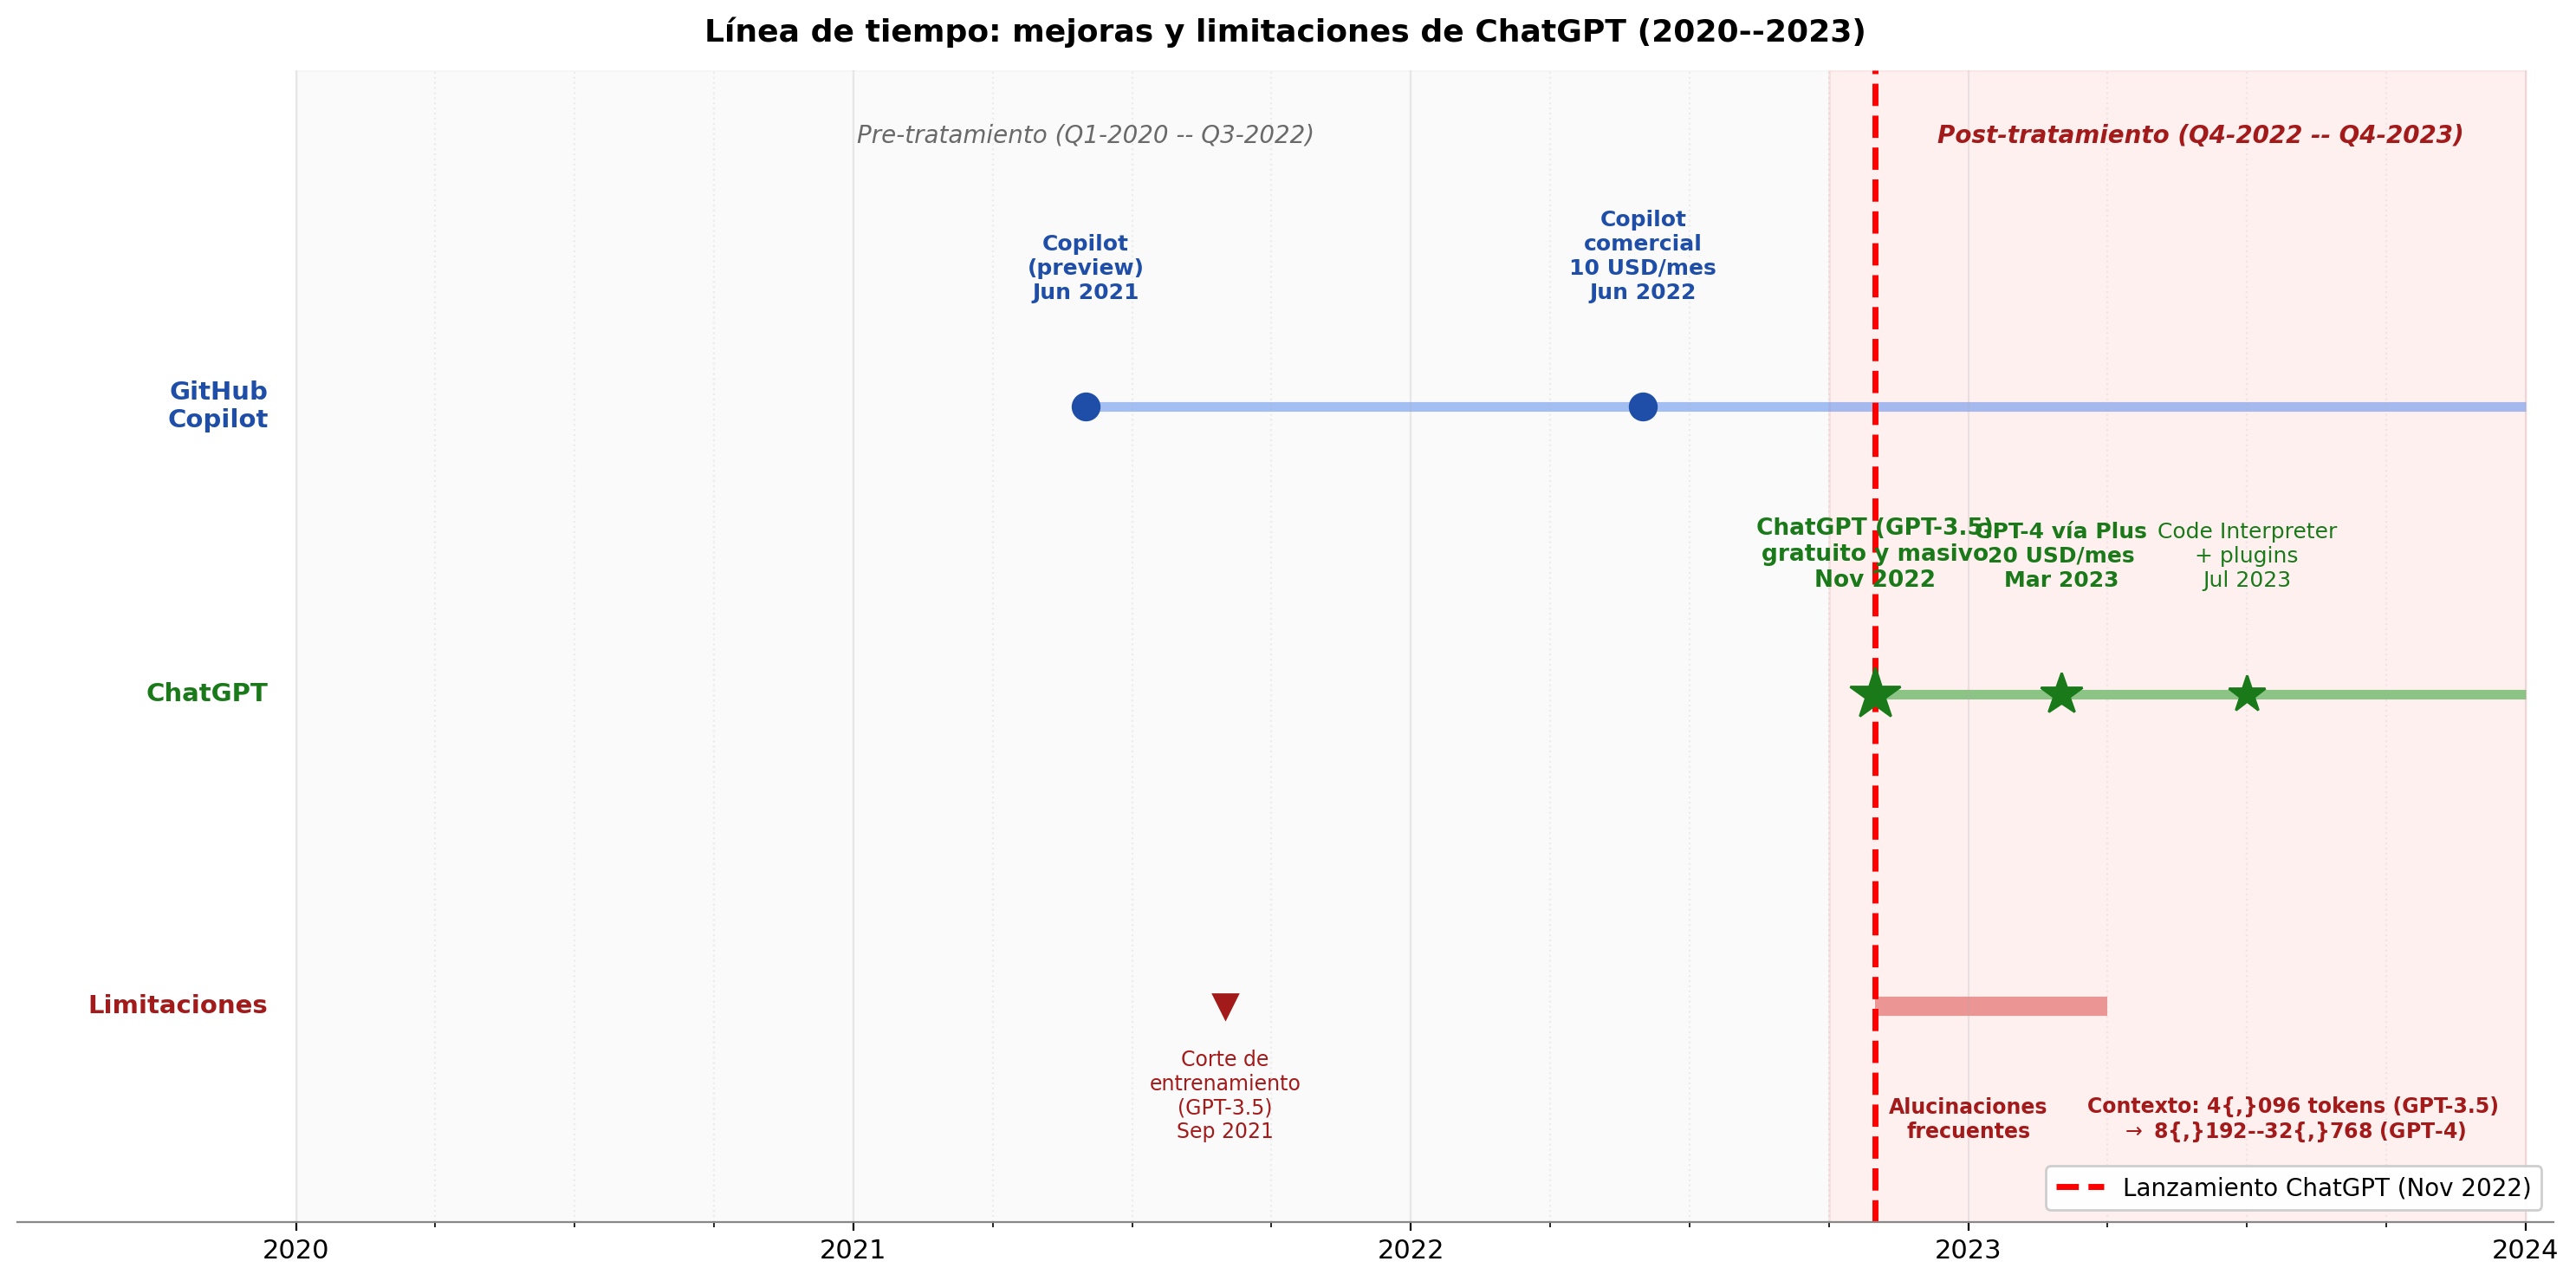
\includegraphics[width=\textwidth,height=0.74\textheight,keepaspectratio]{chatgpt_timeline.png}

\vspace{0.3em}
\footnotesize \textit{Tres carriles:} GitHub Copilot (azul), ChatGPT (verde), Limitaciones (rojo, duraciones).
\end{frame}

\begin{frame}{Implicaciones para la interpretación}
\textbf{La ventana postratamiento (Q4-2022 a Q4-2023) no fue homogénea:}

\begin{columns}[T]
\begin{column}{0.5\textwidth}
\textbf{Q4-2022 -- Q1 2023}
\medskip

\small
\begin{itemize}\small
  \item GPT-3.5 gratuito
  \item Alucinaciones frecuentes
  \item Contexto 4\,096 tokens
  \item Corte de entrenamiento: Sep 2021
\end{itemize}
\end{column}
\begin{column}{0.5\textwidth}
\textbf{Q2-Q4 2023}
\medskip

\small
\begin{itemize}\small
  \item GPT-4 vía Plus (20 USD/mes)
  \item Reducción de alucinaciones
  \item Contexto 8\,192--32\,768 tokens
  \item Code Interpreter, \textit{plugins}
\end{itemize}
\end{column}
\end{columns}

\vspace{1em}
\centering \alert{Esto abre la posibilidad de un efecto no monotónico en el corto plazo.}
\end{frame}

% ════════════════════════════════════════════════════════════════════════════
\section{6. Datos}
% ════════════════════════════════════════════════════════════════════════════

\begin{frame}{Fuente y variable de interés}
\begin{block}{Fuente: GitHub Innovation Graph}
Base pública mantenida por GitHub con métricas agregadas de actividad de desarrollo por país, lenguaje y trimestre.
\end{block}

\textbf{Variable de resultado:} \textit{unique pushers} por cada 100\,000 habitantes.

\medskip

\textit{Unique pushers} = cantidad de desarrolladores únicos que al menos hicieron un \texttt{git push} en GitHub durante un trimestre, normalizado por población.

\vspace{0.5em}
\begin{itemize}
  \item \textbf{Mide:} entrada/persistencia de programadores activos.
  \item \textbf{No mide:} intensidad por persona, calidad del código, valor agregado.
  \item \textbf{Limitación reconocida:} países como China usan plataformas alternativas (Gitee) $\Rightarrow$ posible subestimación en el control.
\end{itemize}
\end{frame}

\begin{frame}{Diseño del panel}
\begin{columns}[T]
\begin{column}{0.55\textwidth}
\textbf{Dimensiones del panel:}
\begin{itemize}
  \item \textbf{159 países} ($N$): 130 tratados + 29 control.
  \item \textbf{10 lenguajes:} C, C\#, C++, Go, Java, JavaScript, PHP, Python, Ruby, TypeScript.
  \item \textbf{16 trimestres:} Q1-2020 a Q4-2023.
  \item \textbf{Total:} 25\,440 observaciones.
\end{itemize}

\medskip
\textbf{Período de pretratamiento:} 12 trimestres (Q1-2020 a Q3-2022).

\textbf{Período de tratamiento:} 4 trimestres (Q4-2022 a Q4-2023).

\medskip
\textbf{Exclusiones:} EU (agregado), Kosovo (sin código ISO procesable), Hong Kong (atípico).
\end{column}
\begin{column}{0.42\textwidth}
\textbf{Países sin acceso a ChatGPT (control)}
\medskip

\scriptsize \textbf{Censores severos}: China, Cuba, Irán, Bielorrusia, Rusia, Siria.

\textbf{Otros}: Afganistán, Bahréin, Burundi, Camboya, Camerún, Congo (RD), Egipto, Eswatini, Etiopía, Guadalupe, Macao, Puerto Rico, Reunión, Somalia, Sudán, Tayikistán, Turkmenistán, Turquía, Uzbekistán, Venezuela, Vietnam, Yemen, Zimbabue, Libia, Laos.
\end{column}
\end{columns}
\end{frame}

\begin{frame}{Mapa global de disponibilidad de ChatGPT}
\centering
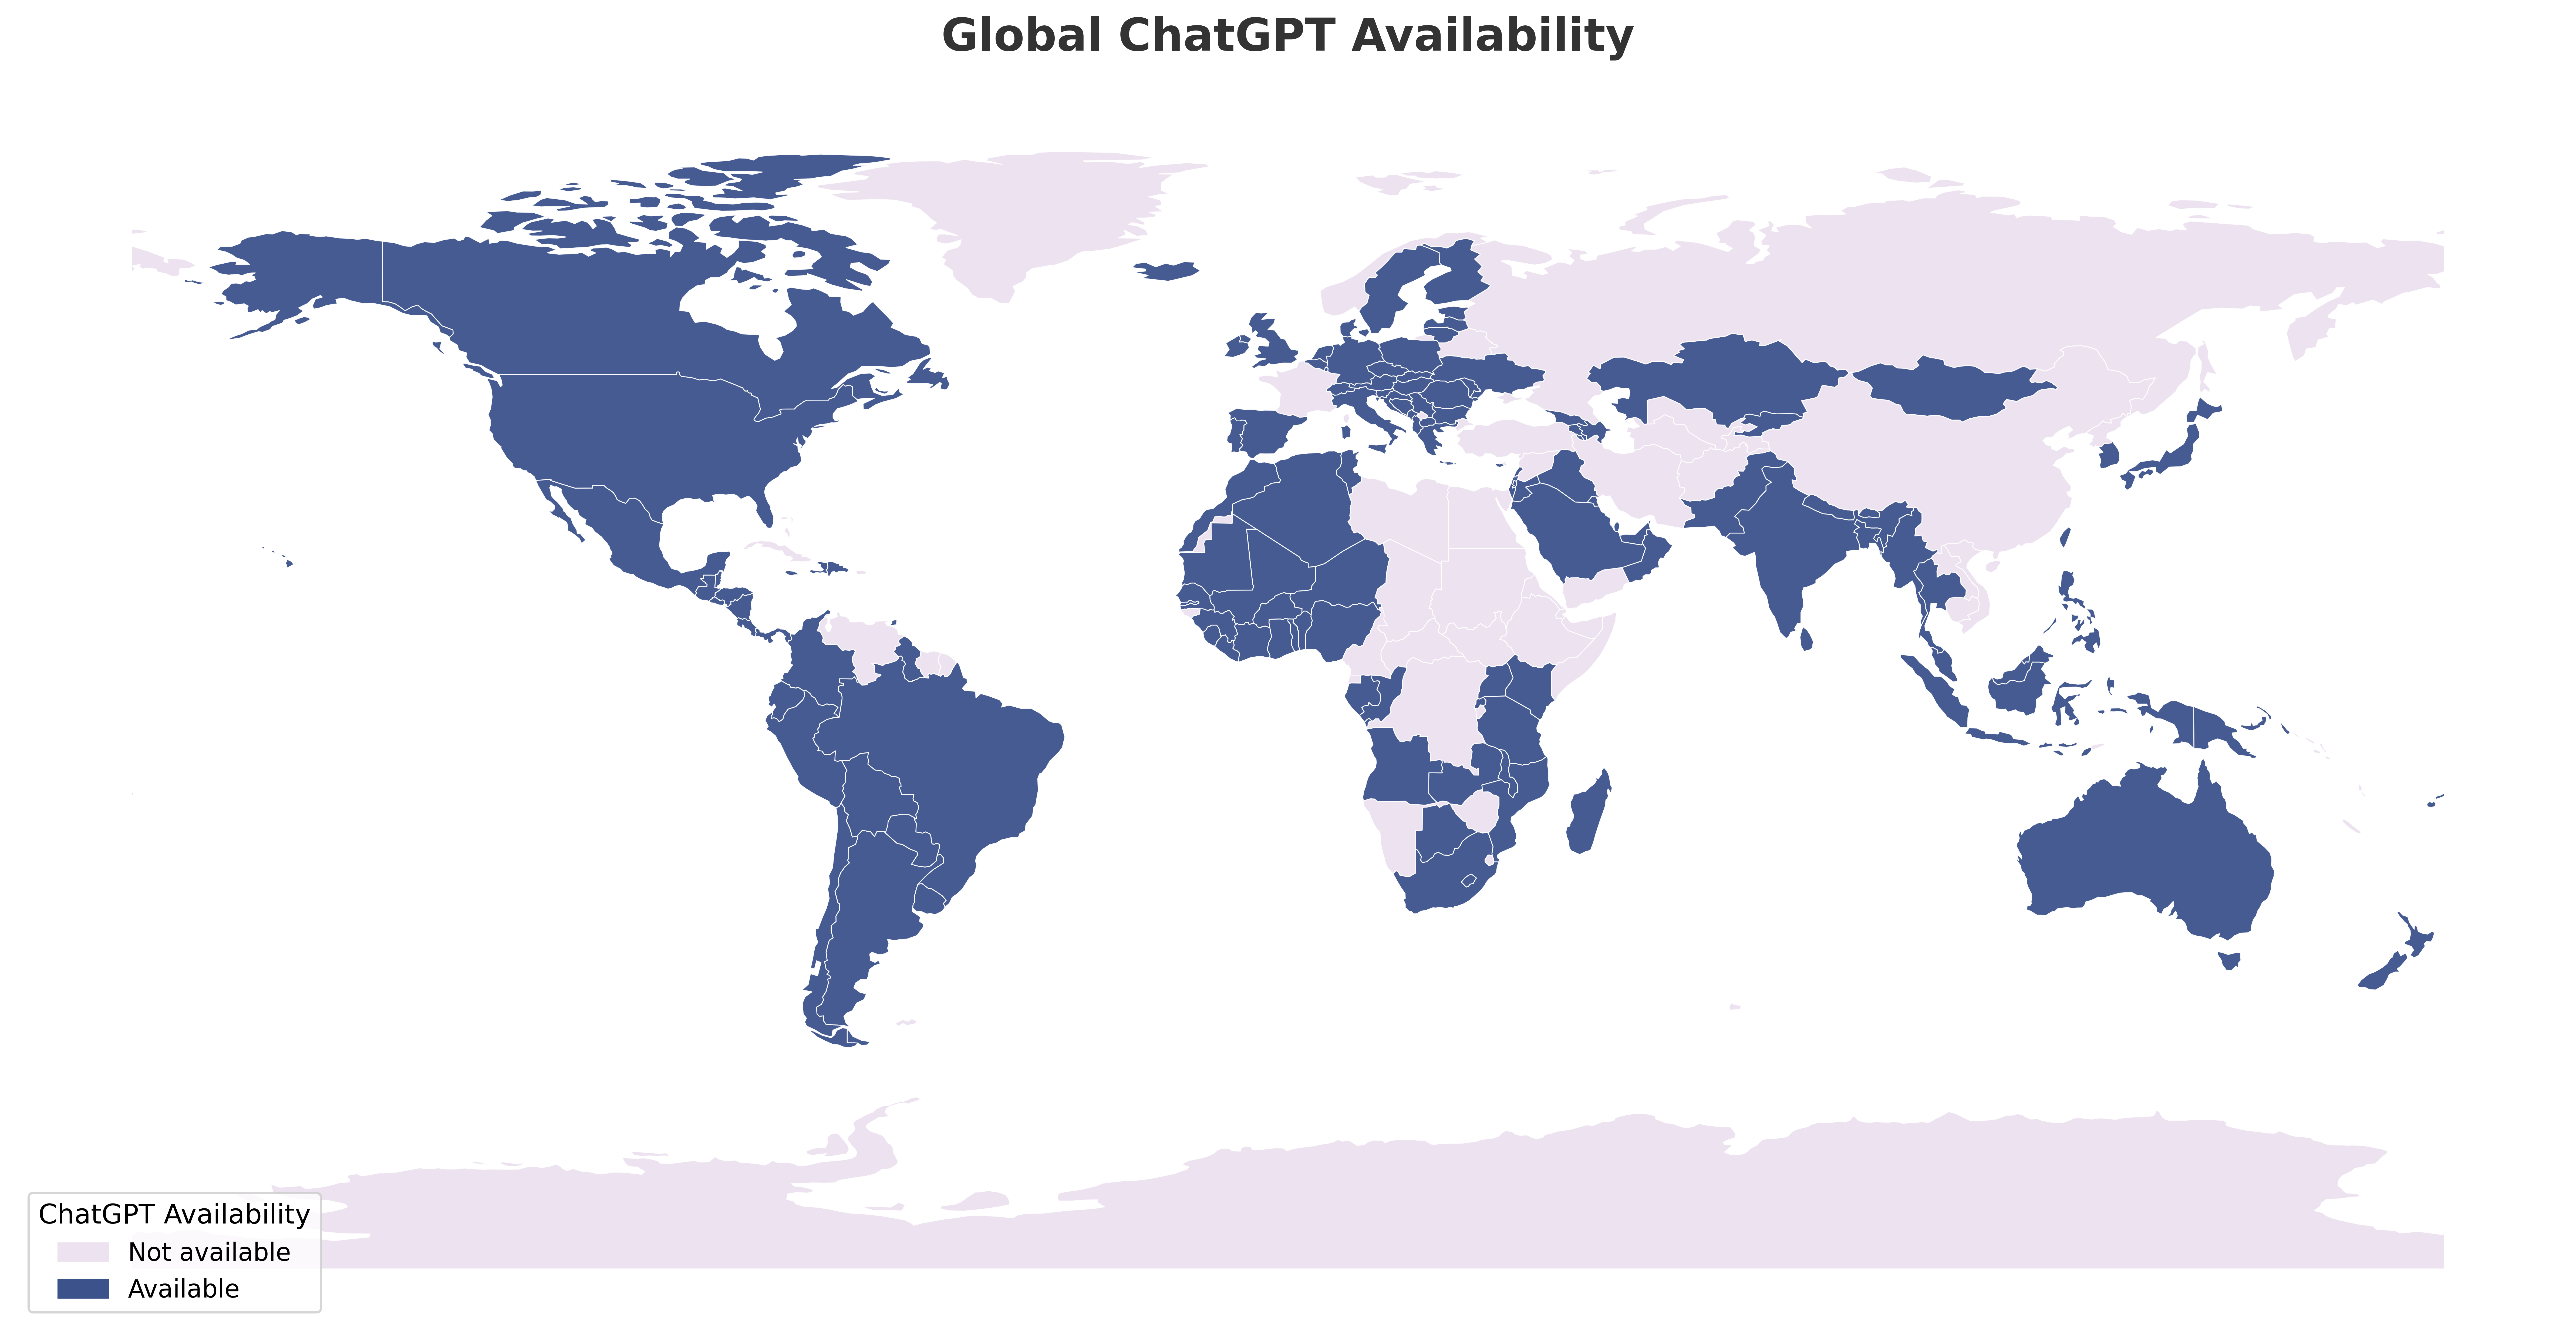
\includegraphics[width=\textwidth,height=0.74\textheight,keepaspectratio]{chatgpt_global_availability_map.png}

\vspace{0.2em}
\footnotesize \textbf{Azul:} países con acceso (tratados, $N=130$). \textbf{Gris claro:} países sin acceso (control, $N=29$).
\end{frame}

\begin{frame}{Estadísticos descriptivos clave}
\renewcommand{\arraystretch}{1.30}
\centering
\textbf{Media de \textit{unique pushers} por 100k habitantes}

\vspace{0.3em}
\small
\begin{tabular}{lcccc}
\toprule
 & \multicolumn{2}{c}{\textbf{Pretratamiento}} & \multicolumn{2}{c}{\textbf{Postratamiento}} \\
 \cmidrule(lr){2-3}\cmidrule(lr){4-5}
\textbf{Lenguaje} & Control & Tratado & Control & Tratado \\
\midrule
JavaScript & 18,84 & 51,00 & 34,29 & 58,98 \\
Python     & 13,30 & 22,71 & 22,21 & 33,46 \\
TypeScript &  3,46 & 17,32 & 11,79 & 18,83 \\
Java       &  6,59 & 13,58 & 10,81 & 16,14 \\
C          &  4,88 &  7,16 &  8,73 & 10,91 \\
C++        &  5,28 &  7,77 &  8,84 & 10,82 \\
C\#        &  3,01 &  7,39 &  4,41 &  9,64 \\
Go         &  1,74 &  3,63 &  4,85 &  4,05 \\
Ruby       &  3,13 &  6,07 &  4,00 &  6,28 \\
PHP        &  2,27 &  7,54 &  3,46 &  8,24 \\
\bottomrule
\end{tabular}

\vspace{0.6em}
\footnotesize \textit{Lectura:} ambos grupos crecen en el período. El efecto causal requiere comparar las \textbf{tasas} de cambio, no los niveles.
\end{frame}

\begin{frame}{Tendencias temporales (países sin ChatGPT)}
\centering
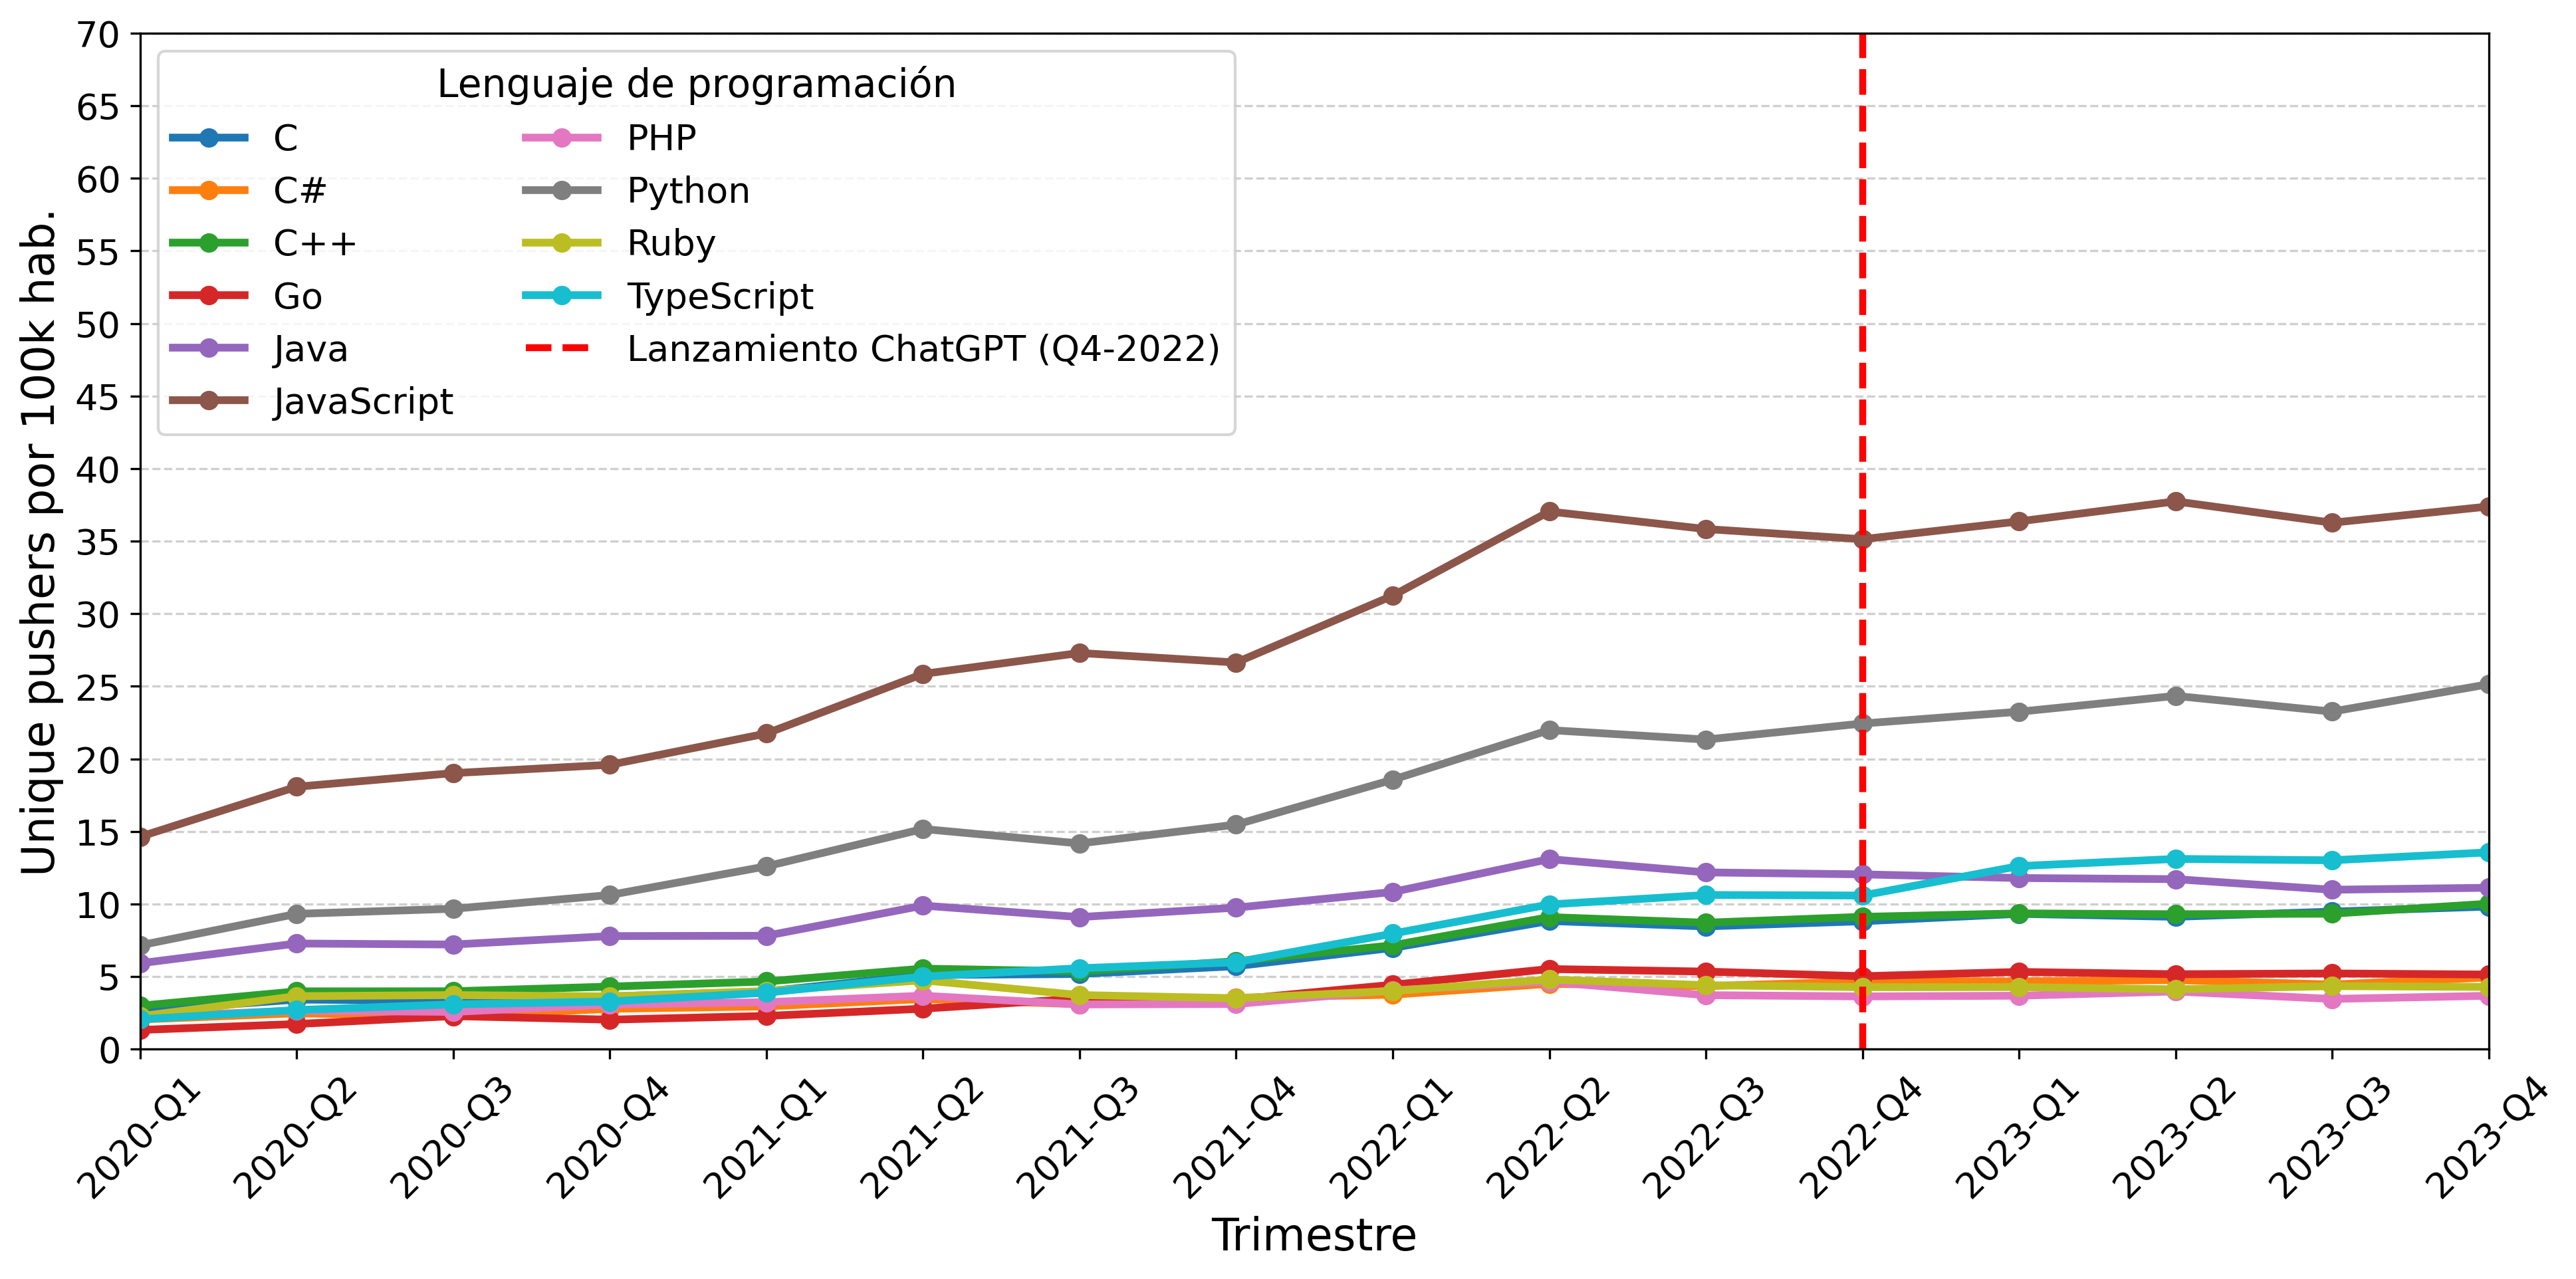
\includegraphics[width=\textwidth,height=0.74\textheight,keepaspectratio]{language_trend_no_gpt_countries_2020_2023.png}

\vspace{0.2em}
\footnotesize Línea vertical roja: lanzamiento de ChatGPT (Q4-2022). \textbf{En el grupo de control las series no muestran aceleración tras el tratamiento.}
\end{frame}

\begin{frame}{Tendencias temporales (países con ChatGPT)}
\centering
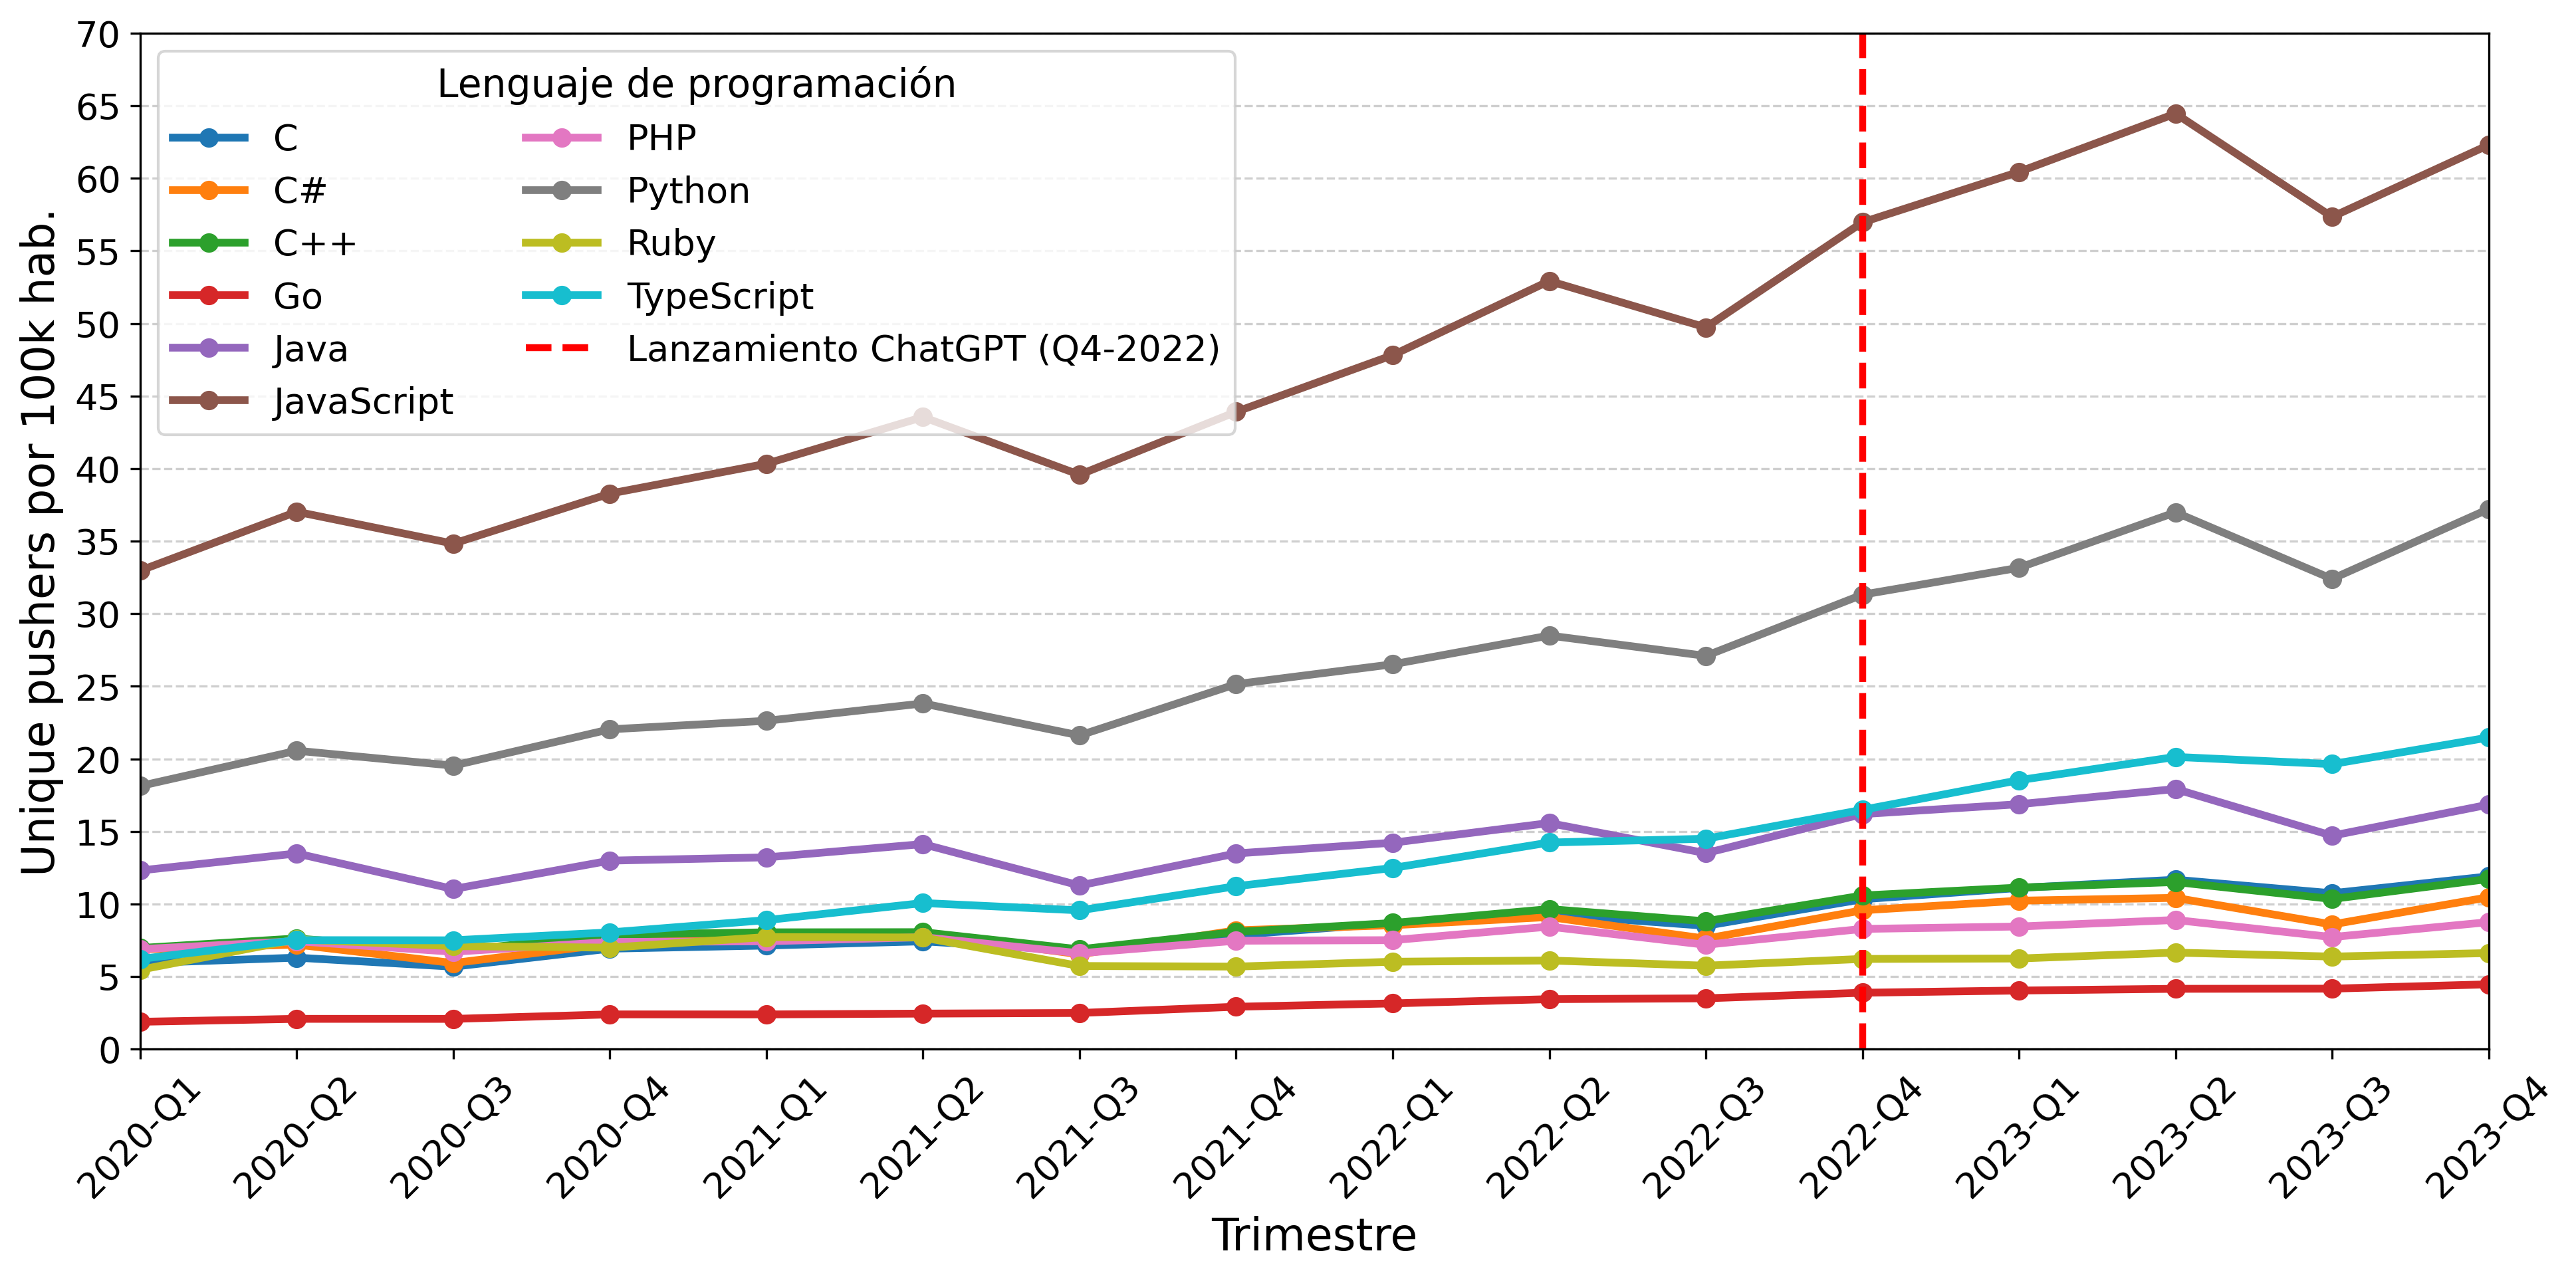
\includegraphics[width=\textwidth,height=0.74\textheight,keepaspectratio]{language_trend_gpt_countries_2020_2023.png}

\vspace{0.2em}
\footnotesize Línea vertical roja: lanzamiento de ChatGPT (Q4-2022). \textbf{Atención a la aceleración de JavaScript, Python y TypeScript post-tratamiento.}
\end{frame}

% ════════════════════════════════════════════════════════════════════════════
\section{7. Metodología}
% ════════════════════════════════════════════════════════════════════════════

\begin{frame}{Marco común: resultados potenciales}
\textbf{Para cada unidad $i$ en el período $t$:}
\[
Y_{it} = Y_{it}^{(0)} + \tau_{it}\, W_{it}
\]

donde $W_{it} = \mathbf{1}\!\left[i \in \mathcal{T},\; t \geq T_0 + 1\right]$.

\medskip
\textbf{Parámetro de interés:} efecto promedio del tratamiento sobre los tratados (ATT):
\[
\tau = \frac{1}{N_{tr}\, T_{post}} \sum_{i \in \mathcal{T}}\sum_{t > T_0} \tau_{it}
\]

\vspace{0.8em}
\begin{block}{Tres estrategias para estimar $\tau$}
\begin{enumerate}
  \item \textbf{DiD} --- Diferencias en Diferencias (Card \& Krueger, 1994).
  \item \textbf{CS} --- Control Sintético (Abadie, Diamond \& Hainmueller, 2010).
  \item \textbf{SDiD} --- Diferencias en Diferencias Sintética (Arkhangelsky et al., 2021). \alert{Método principal.}
\end{enumerate}
\end{block}
\end{frame}

\begin{frame}{Método 1: DiD}
\textbf{Especificación de efectos fijos de dos vías:}
\[
Y_{it} = \mu + \alpha_i + \beta_t + \tau^{DiD}\, W_{it} + \varepsilon_{it}
\]

\medskip
\textbf{Estimador explícito:}
\[
\hat{\tau}^{DiD} = \bigl(\bar{Y}_{post,\,\mathcal{T}} - \bar{Y}_{pre,\,\mathcal{T}}\bigr) - \bigl(\bar{Y}_{post,\,\mathcal{C}} - \bar{Y}_{pre,\,\mathcal{C}}\bigr)
\]

\vspace{0.5em}
\textbf{Supuesto crítico:} tendencias paralelas pre-tratamiento.

\textbf{Debilidad para este estudio:} el control es heterogéneo (países autoritarios) y las tendencias pretratamiento podrían no ser paralelas.
\end{frame}

\begin{frame}{Método 2: Control Sintético (CS)}
\textbf{Estimador:}
\[
\hat{\tau}^{SC} = \frac{1}{N_{tr}\,T_{post}} \sum_{i \in \mathcal{T}}\sum_{t > T_0} \left(Y_{it} - \sum_{j \in \mathcal{C}} \hat{\omega}_j^{sc}\,Y_{jt}\right)
\]

\textbf{Pesos $\hat{\omega}_j^{sc}$:}
\[
\hat{\boldsymbol{\omega}}^{sc} = \arg\min_{\boldsymbol{\omega}}\;\sum_{t=1}^{T_0} \left(\sum_{j \in \mathcal{C}} \omega_j\,Y_{jt} - \bar{Y}_t^{\mathcal{T}}\right)^{\!2}
\quad \text{s.a.} \quad \omega_j \geq 0,\; \sum_j \omega_j = 1
\]

\vspace{0.5em}
\textbf{Idea:} construir un ``tratado sintético'' como promedio ponderado de los controles, que copie la trayectoria pretratamiento del tratado real.

\textbf{Ventaja:} maneja heterogeneidad en el grupo de control.

\textbf{Limitación:} mayor varianza cuando el tratado es agregado de muchas unidades heterogéneas.
\end{frame}

\begin{frame}{Método 3: SDiD (Arkhangelsky et al., 2021)}
\textbf{Combina DiD y CS asignando pesos a unidades \textbf{y} a períodos:}
\[
(\hat{\tau}^{sdid},\,\hat{\mu},\,\hat{\alpha},\,\hat{\beta}) = \arg\min \sum_{i,t} \hat{\omega}_i^{sdid}\,\hat{\lambda}_t^{sdid} \bigl(Y_{it} - \mu - \alpha_i - \beta_t - W_{it}\,\tau\bigr)^2
\]

\textbf{Pesos unitarios $\hat{\boldsymbol{\omega}}^{sdid}$:} resuelven un problema CS con regularización.

\textbf{Pesos temporales $\hat{\boldsymbol{\lambda}}^{sdid}$:} dan más peso a períodos pretratamiento cercanos a $T_0$.

\vspace{0.5em}
\begin{block}{Por qué SDiD es el principal}
\begin{itemize}
  \item Asintóticamente normal con muchas unidades tratadas ($N_{tr} = 130$).
  \item Robusto a violaciones del supuesto de tendencias paralelas.
  \item Combina la flexibilidad de CS con la simplicidad de DiD.
\end{itemize}
\end{block}
\end{frame}

\begin{frame}{Inferencia y pruebas de robustez}
\textbf{Inferencia: \textit{bootstrap} por remuestreo de unidades.}
\begin{itemize}
  \item DiD y SDiD: 100 replicaciones.
  \item CS: 2\,000 replicaciones (mayor varianza por iteración).
\end{itemize}

\vspace{0.5em}
\textbf{Pruebas de robustez adicionales:}
\begin{enumerate}
  \item \textbf{Cuadro 4:} con variables de control (uso de PC y de internet, Banco Mundial).
  \item \textbf{Cuadro 5:} grupo de control restringido (excluye los 6 censores severos de Freedom House).
  \item \textbf{Cuadro 6:} \alert{placebos in-space + sensibilidad LOO al pool de donantes} (Abadie, 2010, 2021).
\end{enumerate}
\end{frame}

% ════════════════════════════════════════════════════════════════════════════
\section{8. Resultados}
% ════════════════════════════════════════════════════════════════════════════

\begin{frame}{Resultados principales: ATT por método (Cuadro 3)}
\vspace{0.2em}
\renewcommand{\arraystretch}{1.22}
\setlength{\tabcolsep}{8pt}
\centering
\footnotesize
\begin{tabular}{lccc}
\toprule
\textbf{Lenguaje} & \textbf{DiD} & \textbf{CS} & \textbf{SDiD} \\
\midrule
\textbf{JavaScript} & 13,635*** \,(2,719) & 9,451*  \,(5,307) & \alert{\textbf{8,303***}} \,(3,180) \\
\textbf{Python}     &  7,688*** \,(1,193) & 1,604   \,(3,552) & \alert{\textbf{4,525***}} \,(1,321) \\
\textbf{TypeScript} &  7,181*** \,(0,832) & 3,263   \,(2,290) & \alert{\textbf{3,078***}} \,(0,873) \\
\textbf{Java}       &  2,810*** \,(0,827) & 2,206   \,(2,089) & \alert{\textbf{1,725**}}  \,(0,872) \\
\textbf{C}          &  2,689*** \,(0,365) & 1,634   \,(1,137) & \alert{\textbf{1,276***}} \,(0,451) \\
\textbf{C++}        &  2,210*** \,(0,417) & 1,212   \,(0,959) & \alert{\textbf{1,131***}} \,(0,435) \\
\textbf{C\#}        &  1,499*** \,(0,381) & 1,001   \,(1,263) & \alert{\textbf{0,443}}    \,(0,379) \\
\textbf{Go}         &  1,411*** \,(0,177) & 0,686   \,(0,606) & \alert{\textbf{0,720***}} \,(0,269) \\
\textbf{PHP}        &  0,904*   \,(0,507) & 1,078   \,(1,013) & \alert{\textbf{0,916**}}  \,(0,465) \\
\textbf{Ruby}       &  0,262    \,(0,266) & 1,521   \,(0,946) & \alert{\textbf{0,808***}} \,(0,274) \\
\bottomrule
\end{tabular}

\vspace{0.5em}
\footnotesize Errores estándar \textit{bootstrap} entre paréntesis. \quad * p$<$0,10 \quad ** p$<$0,05 \quad *** p$<$0,01.
\end{frame}

\begin{frame}{Hallazgos clave del Cuadro 3}
\begin{itemize}
  \item \textbf{Nueve de diez lenguajes} muestran ATT positivo y significativo en el SDiD (1\,\% o 5\,\%).
  \item El único lenguaje sin efecto: \textbf{C\#} (SDiD $= 0{,}443$, no significativo).
  \item Magnitudes más grandes: \textbf{JavaScript} ($+8{,}3$), \textbf{Python} ($+4{,}5$), \textbf{TypeScript} ($+3{,}1$).
  \item Lenguajes con mayor representación en la web y data science presentan mayores efectos $\Rightarrow$ consistente con la \textbf{H2}.
\end{itemize}

\vspace{1em}
\begin{exampleblock}{Pero hay que ser cuidadosos}
La significancia \textit{bootstrap} no es la única evidencia que conviene revisar. Las pruebas de placebo refinan la lectura $\Rightarrow$ siguiente sección.
\end{exampleblock}
\end{frame}

\begin{frame}{Tendencias y contrafactual: Python}
\centering
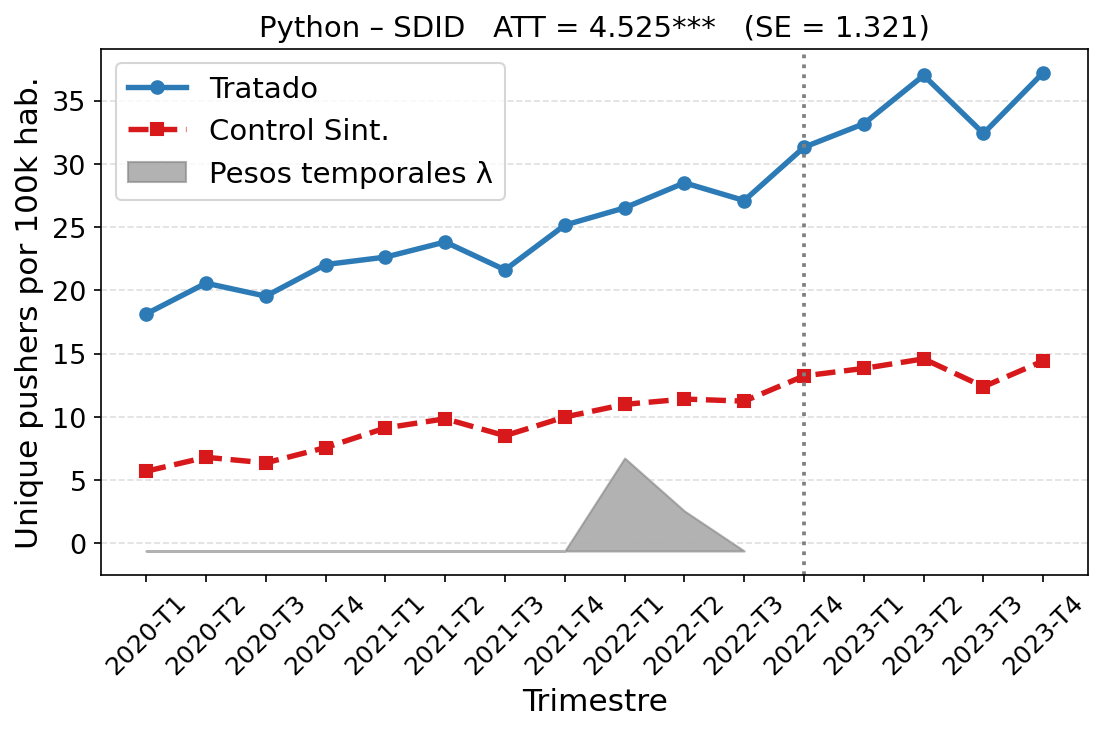
\includegraphics[width=\textwidth,height=0.74\textheight,keepaspectratio]{Pythonsdidtrends12.png}

\vspace{0.2em}
\footnotesize Tratado (azul) vs. control sintético SDiD (rojo). Las trayectorias coinciden hasta Q4-2022; luego divergen. \textbf{ATT $= 4{,}525$} unique pushers por 100k.
\end{frame}

\begin{frame}{Pesos del control sintético: Python}
\centering
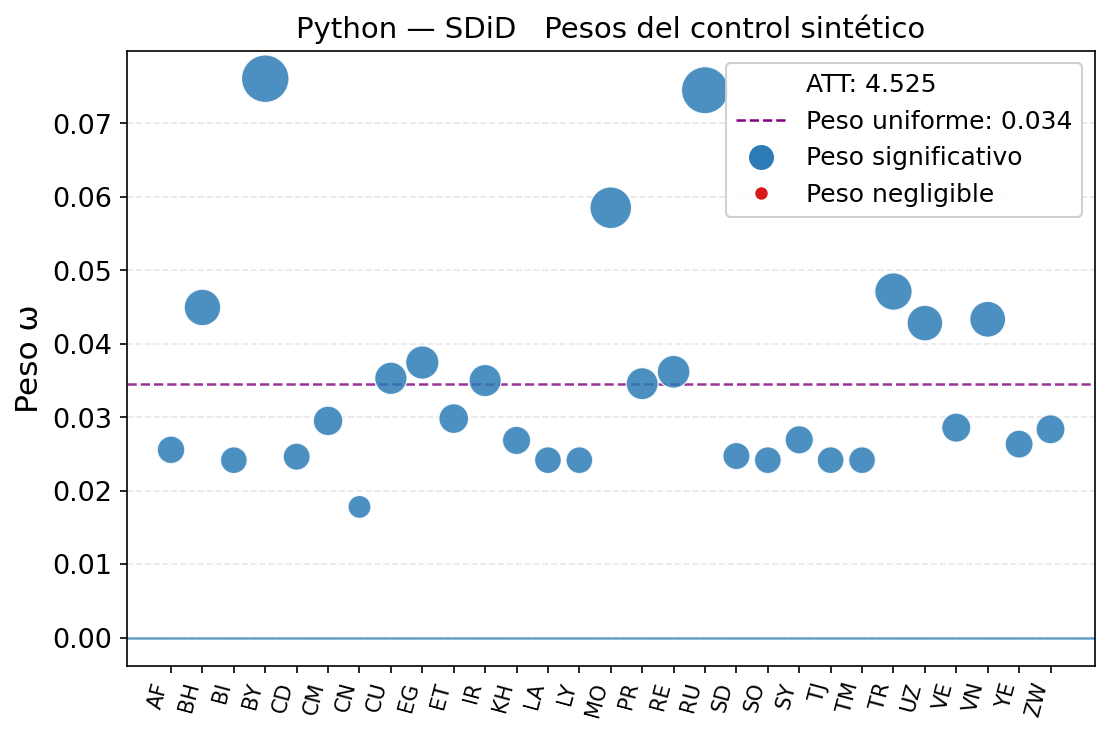
\includegraphics[width=\textwidth,height=0.74\textheight,keepaspectratio]{Pythonsdidweights12.png}

\vspace{0.2em}
\footnotesize \textbf{Puntos azules:} donantes con peso significativo ($\geq 30\,\%$ del peso uniforme). \textbf{Puntos rojos:} pesos negligibles. Línea morada: peso uniforme $1/N_c \approx 0{,}034$.
\end{frame}

\begin{frame}{Tendencias y contrafactual: JavaScript}
\centering
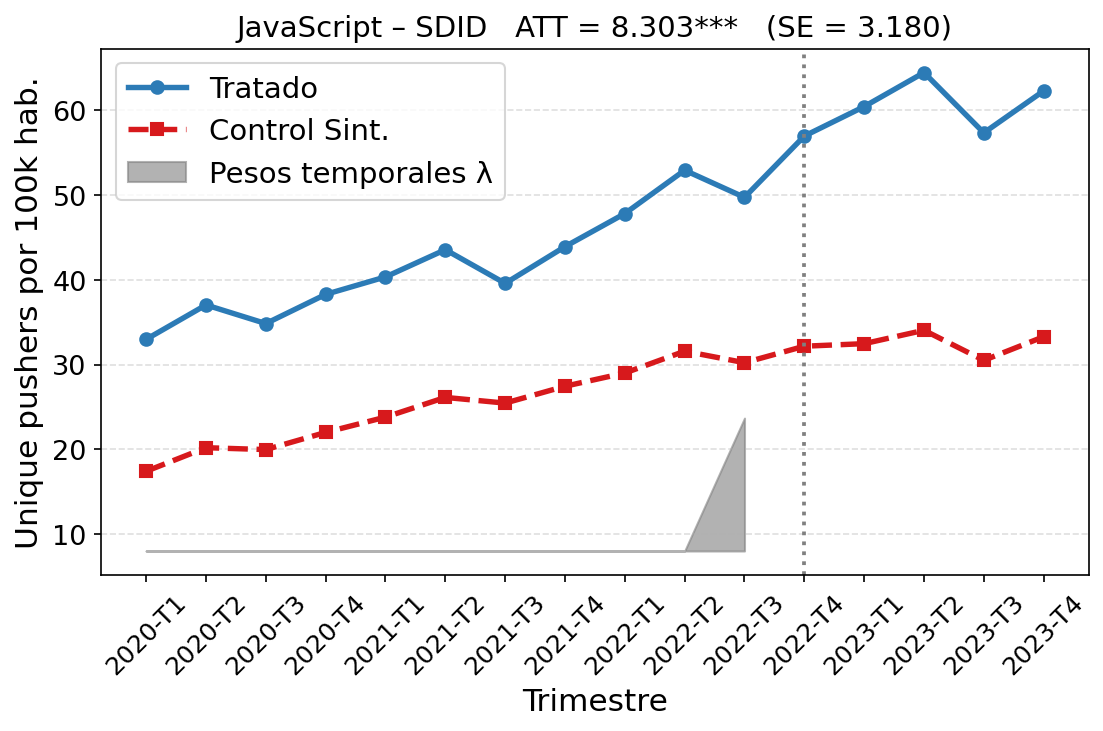
\includegraphics[width=\textwidth,height=0.74\textheight,keepaspectratio]{JavaScriptsdidtrends12.png}

\vspace{0.2em}
\footnotesize \alert{\textbf{Atención:}} ligera pre-tendencia ascendente antes de Q4-2022 $\Rightarrow$ el efecto causal en JavaScript debe interpretarse con cautela pese a la alta significancia.
\end{frame}

% ════════════════════════════════════════════════════════════════════════════
\section{9. Robustez}
% ════════════════════════════════════════════════════════════════════════════

\begin{frame}{Robustez (1): grupo de control restringido}
\textbf{Cuadro 5:} se excluyen los 6 censores severos (CN, CU, IR, BY, RU, SY).

\vspace{0.3em}
\renewcommand{\arraystretch}{1.30}
\centering
\small
\begin{tabular}{lcc}
\toprule
\textbf{Lenguaje} & \textbf{SDiD completo} & \textbf{SDiD restringido} \\
\midrule
\textbf{JavaScript} & 8,303*** & 8,143*** \\
\textbf{Python}     & 4,525*** & 4,378*** \\
\textbf{TypeScript} & 3,078*** & 3,025*** \\
\textbf{Java}       & 1,725**  & 1,734** \\
\textbf{C}          & 1,276*** & 1,235*** \\
\textbf{C++}        & 1,131*** & 1,094*** \\
\textbf{PHP}        & 0,916**  & 0,893** \\
\textbf{Ruby}       & 0,808*** & 0,781*** \\
\textbf{Go}         & 0,720*** & 0,701*** \\
\textbf{C\#}        & 0,443    & 0,398 \\
\bottomrule
\end{tabular}

\vspace{0.4em}
\centering \alert{\textbf{Los resultados son cualitativa y cuantitativamente similares.}}
\end{frame}

\begin{frame}{Robustez (2): placebos in-space y LOO}
\textbf{Cuadro 6:} dos pruebas no paramétricas por lenguaje.

\vspace{0.2em}
\renewcommand{\arraystretch}{1.28}
\setlength{\tabcolsep}{5pt}
\centering
\footnotesize
\begin{tabular}{lccccc}
\toprule
\textbf{Lenguaje} & \textbf{ATT obs.} & \textbf{Media plac.} & \textbf{p-valor plac.} & \textbf{LOO mín} & \textbf{LOO máx} \\
\midrule
\textbf{JavaScript} & 8,303 &  $-0,161$ & \alert{0,069} & 4,642 & 9,322 \\
\textbf{Python}     & 4,525 &   0,355   & \alert{0,069} & 3,553 & 5,111 \\
\textbf{TypeScript} & 3,078 &   0,022   & \alert{0,069} & 1,904 & 3,598 \\
\textbf{Java}       & 1,725 &  $-0,065$ & 0,103         & 1,072 & 2,646 \\
\textbf{C}          & 1,276 &   0,039   & 0,103         & 1,095 & 1,436 \\
\textbf{C++}        & 1,131 &   0,071   & 0,138         & 1,016 & 1,278 \\
\textbf{PHP}        & 0,916 &  $-0,243$ & 0,172         & 0,415 & 1,124 \\
\textbf{Ruby}       & 0,808 &  $-0,009$ & \alert{\textbf{0,034}} & 0,667 & 0,853 \\
\textbf{Go}         & 0,720 &  $-0,007$ & \alert{\textbf{0,034}} & 0,587 & 0,839 \\
\textbf{C\#}        & 0,443 &  $-0,010$ & 0,207         & 0,411 & 0,824 \\
\bottomrule
\end{tabular}

\vspace{0.4em}
\footnotesize Placebos in-space: 29 placebos por lenguaje. LOO: 29 reestimaciones eliminando un control a la vez.
\end{frame}

\begin{frame}{Tres niveles de evidencia}
\begin{columns}[T]
\begin{column}{0.32\textwidth}
\textbf{\textcolor{pucpblue}{Fuerte (p $\leq$ 0,05)}}
\medskip

\begin{itemize}\small
  \item Go (p $= 0{,}034$)
  \item Ruby (p $= 0{,}034$)
\end{itemize}
\medskip

ATT atípico vs. placebos.
\end{column}
\begin{column}{0.32\textwidth}
\textbf{\textcolor{orange!80!black}{Moderada (p $\leq$ 0,10)}}
\medskip

\begin{itemize}\small
  \item JavaScript (0,069)
  \item Python (0,069)
  \item TypeScript (0,069)
\end{itemize}
\medskip

Lenguajes priorizados por la hipótesis.
\end{column}
\begin{column}{0.32\textwidth}
\textbf{\textcolor{pucpaccent}{Débil (p $>$ 0,10)}}
\medskip

\begin{itemize}\small
  \item C, C++, Java
  \item PHP
  \item C\#
\end{itemize}
\medskip

Cautela en interpretación causal.
\end{column}
\end{columns}

\vspace{1em}
\begin{block}{Lectura honesta}
La significancia \textit{bootstrap} para C, C++ y Java coexiste con p-valores placebo $> 0{,}10$. Esto sugiere heterogeneidad estructural no completamente absorbida por el contrafactual.
\end{block}
\end{frame}

\begin{frame}{Forest plot: visualización conjunta}
\centering
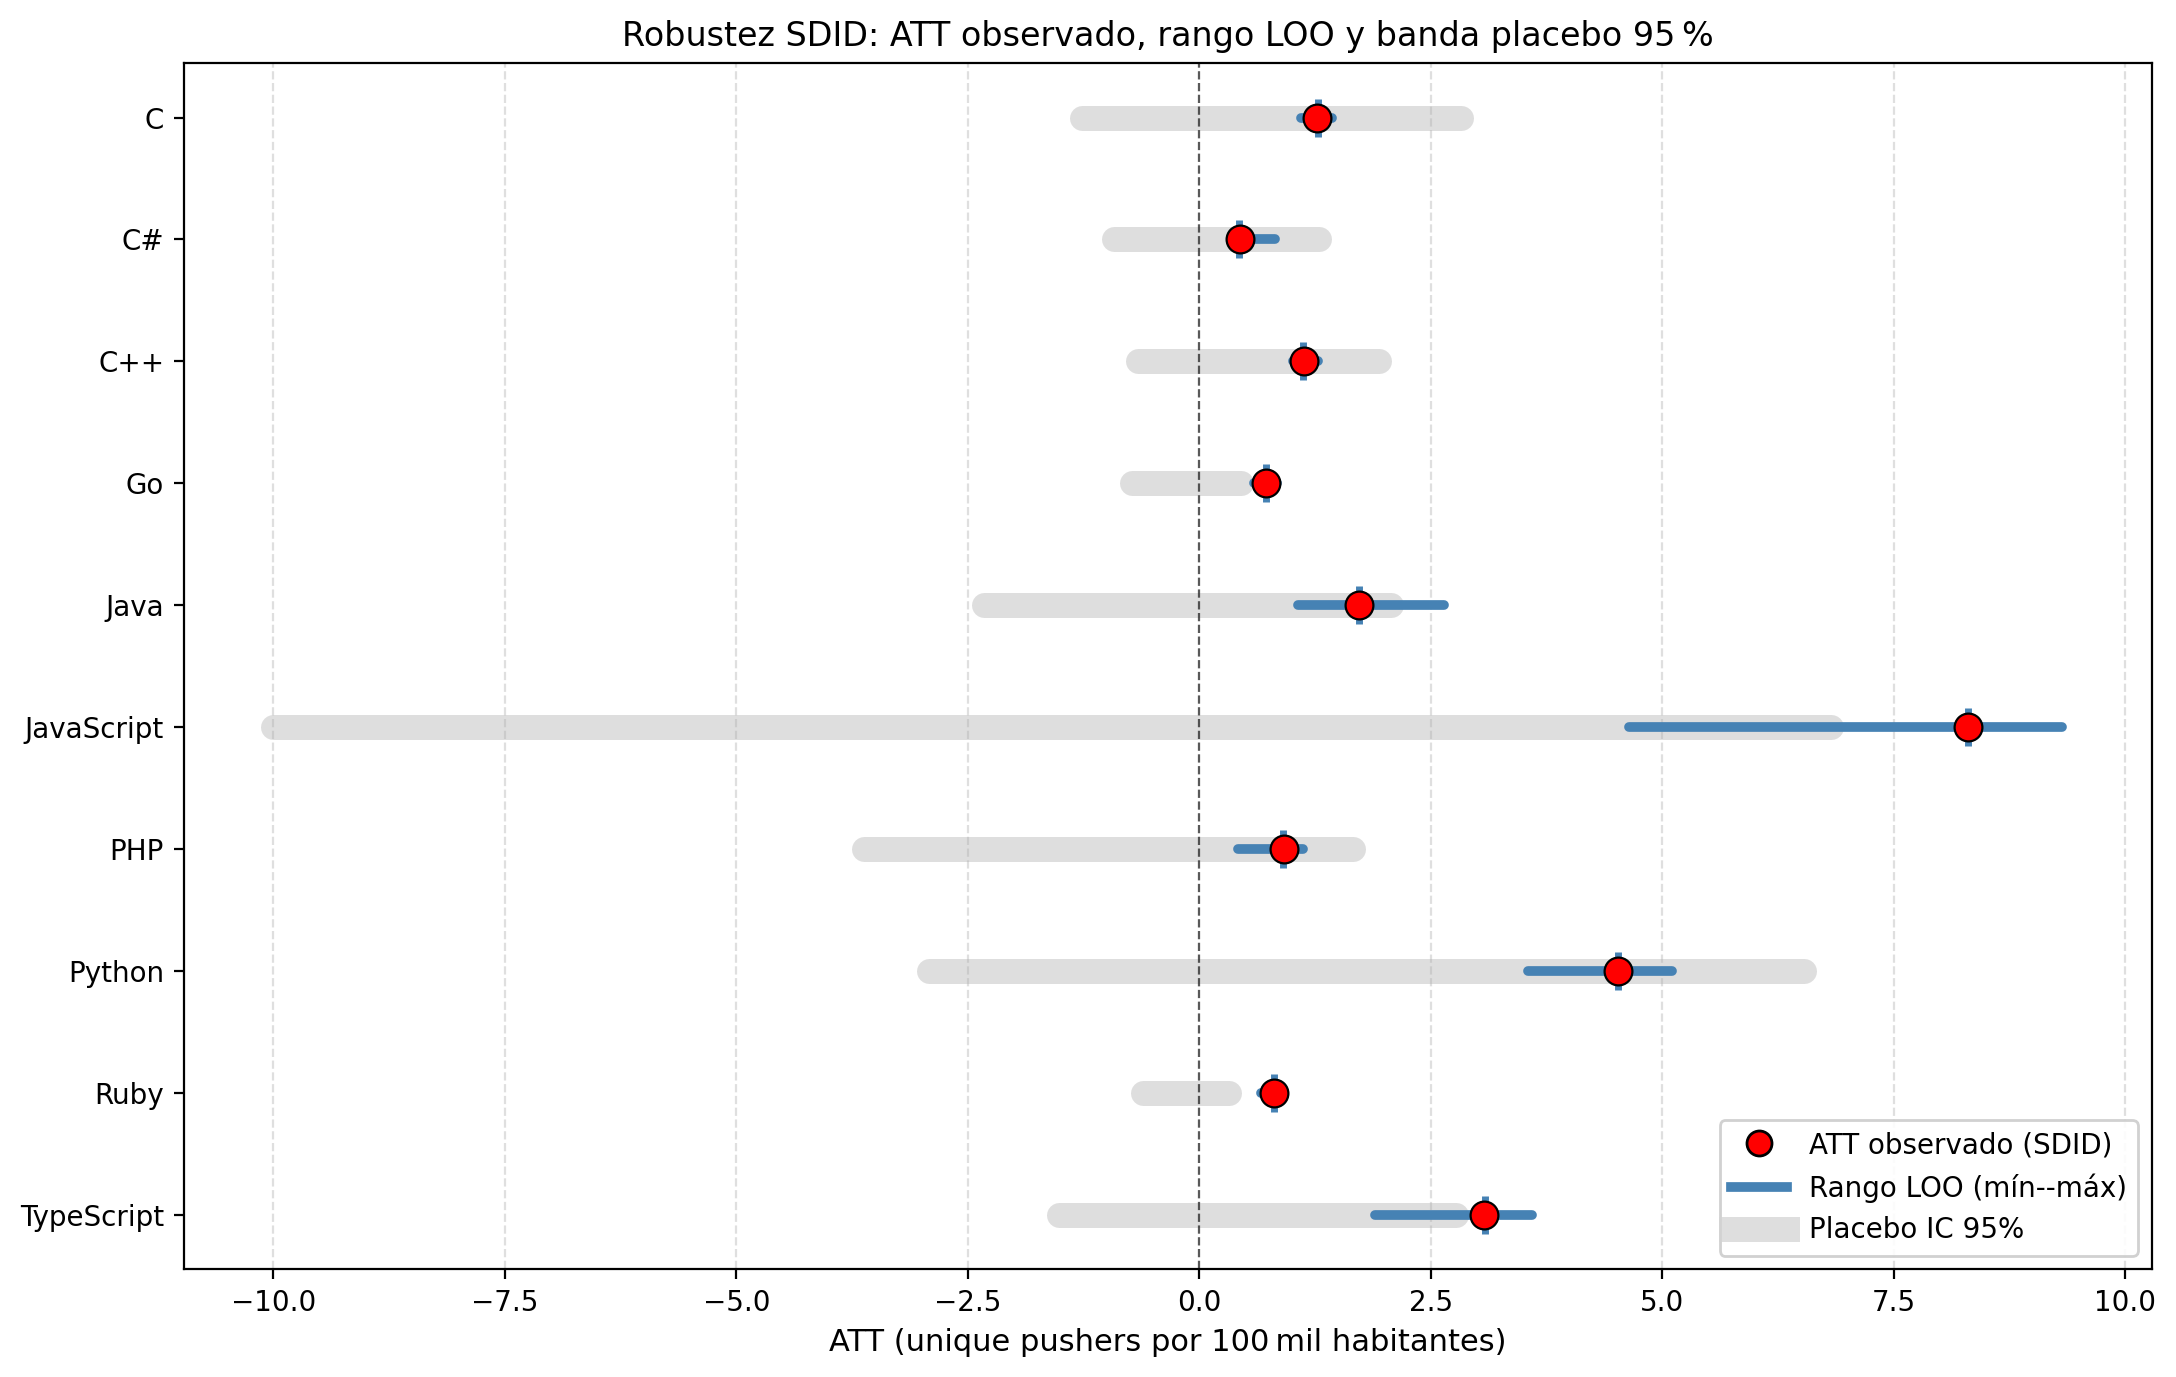
\includegraphics[height=0.78\textheight,keepaspectratio]{robustness_forest_plot.png}

\vspace{0.1em}
\footnotesize \textbf{Punto rojo:} ATT observado. \quad \textbf{Barra azul:} rango LOO. \quad \textbf{Banda gris:} intervalo placebo 95\,\%.
\end{frame}

\begin{frame}{Distribución placebo: 4 lenguajes representativos}
\centering
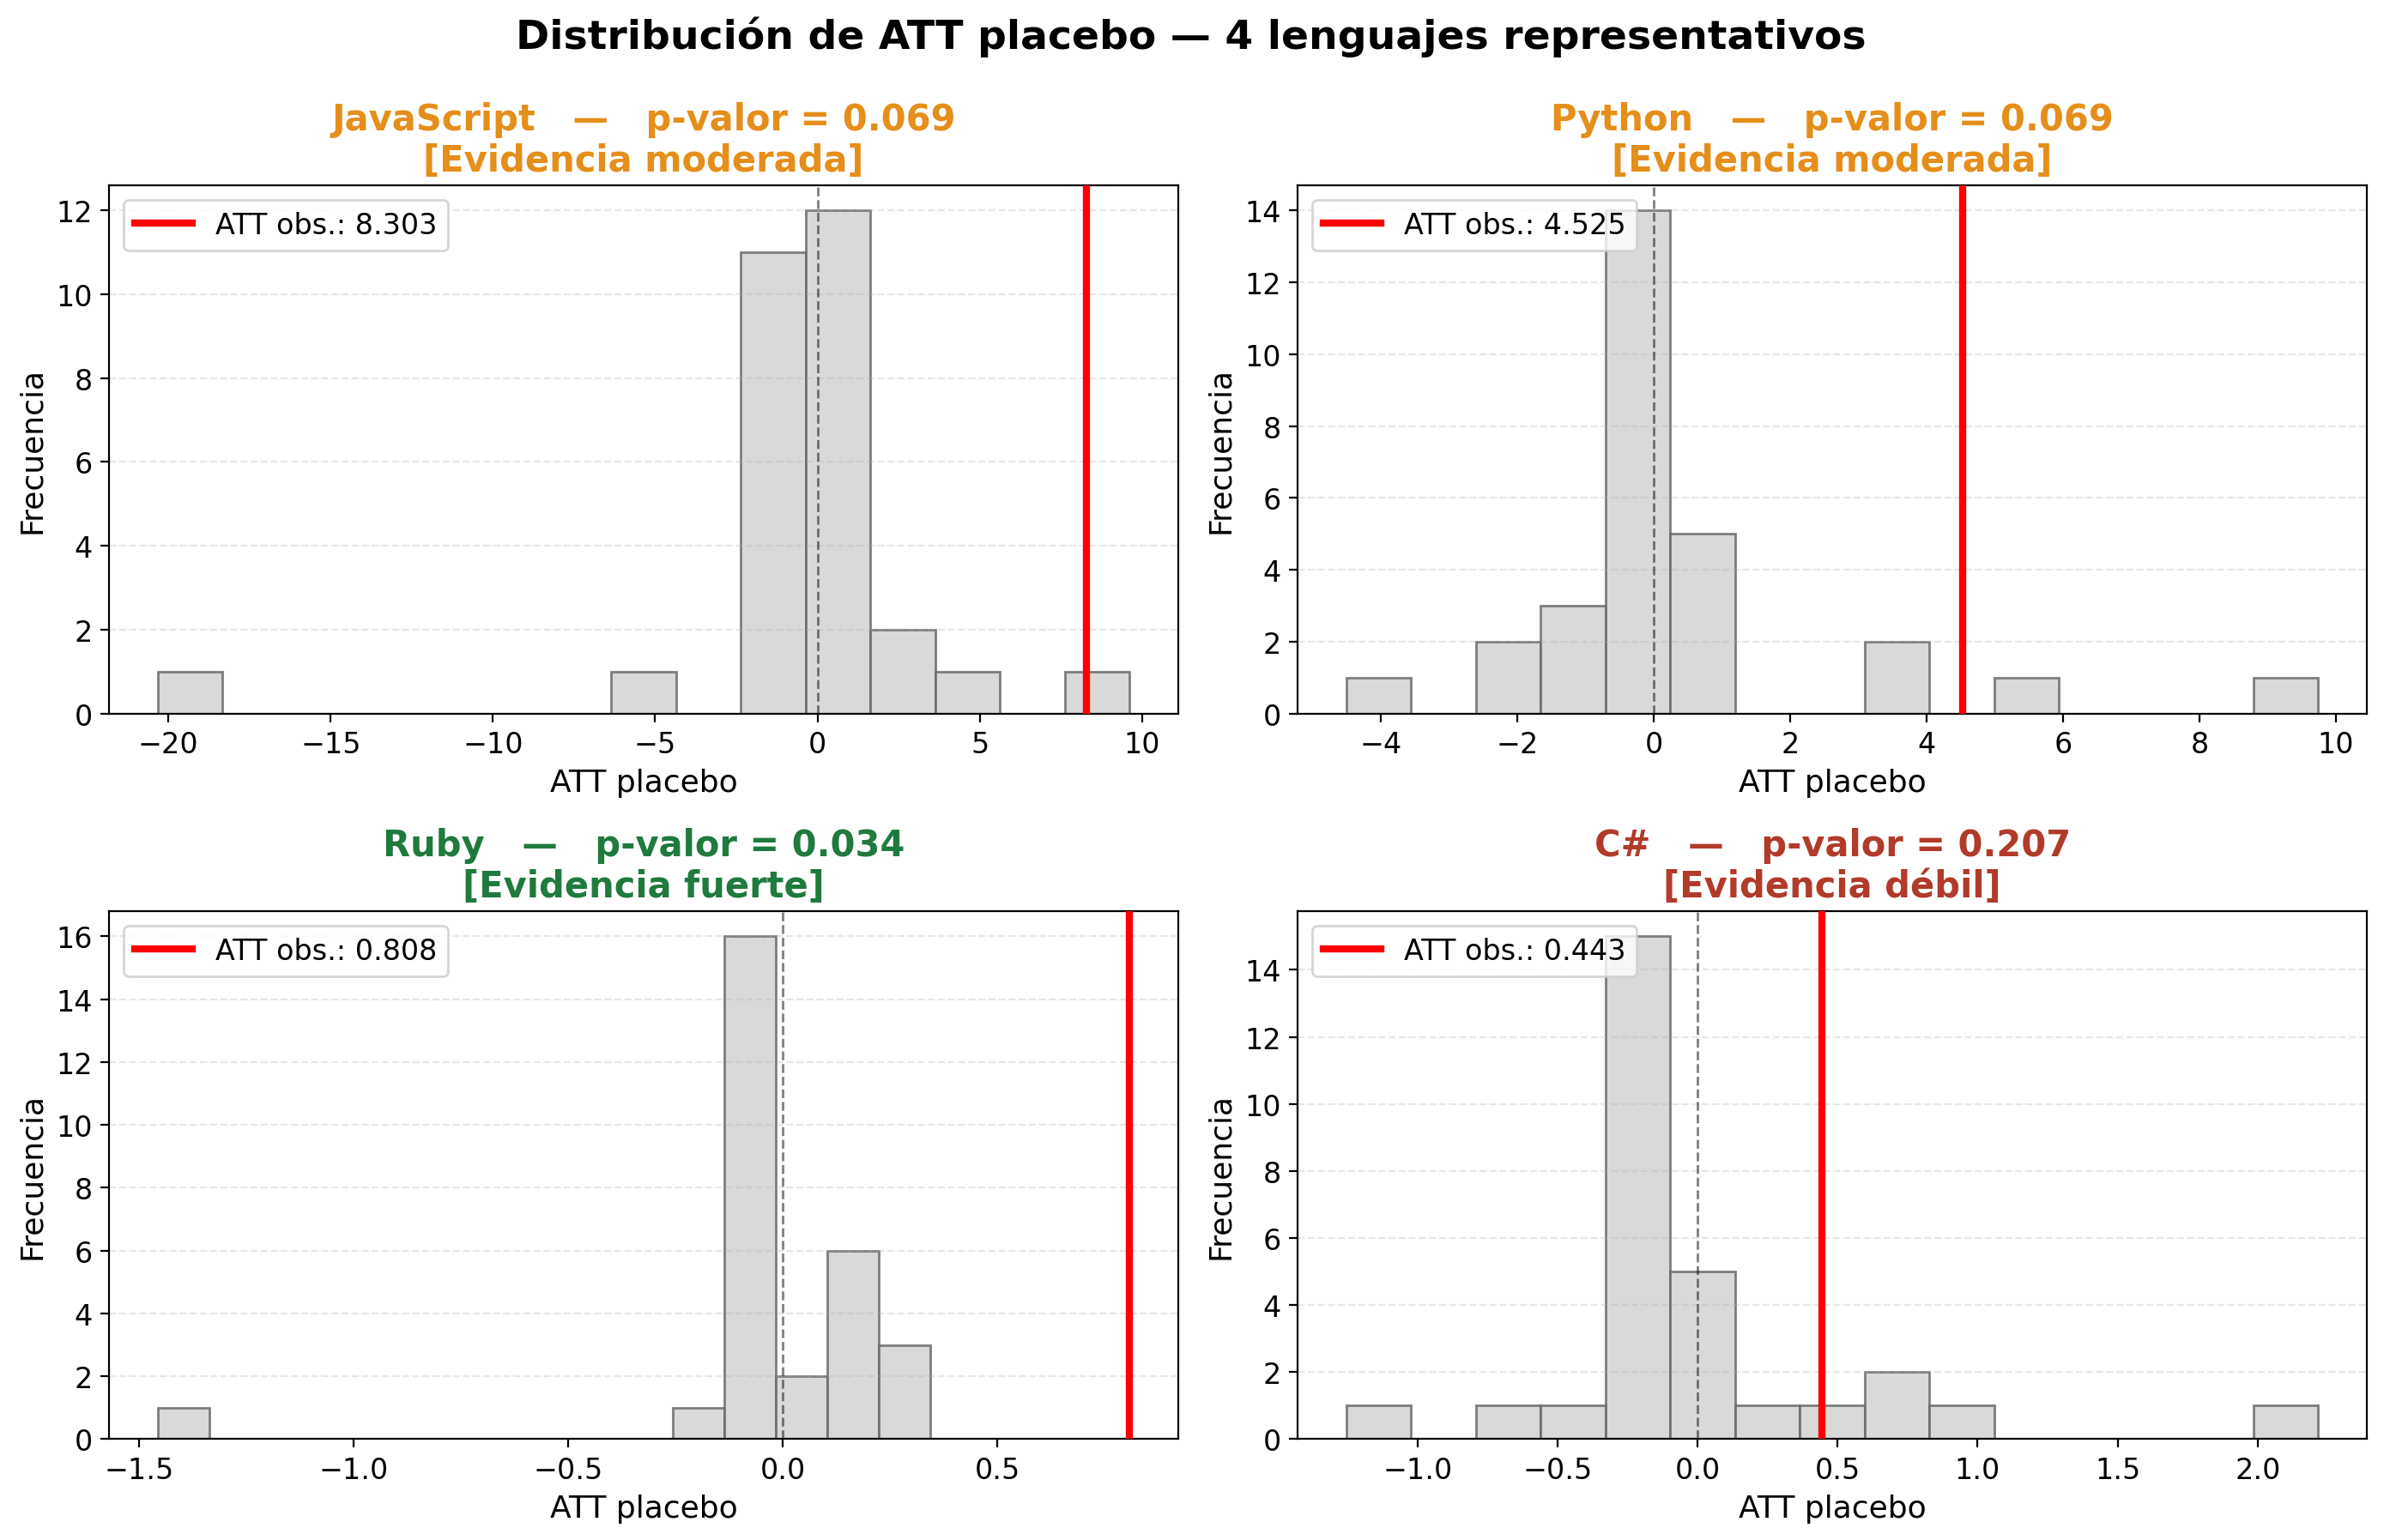
\includegraphics[height=0.80\textheight,keepaspectratio]{placebo_panel_slides.png}

\vspace{0.1em}
\footnotesize Línea roja: ATT observado. \quad Histograma gris: 29 ATT placebo construidos en el grupo de control.
\end{frame}

% ════════════════════════════════════════════════════════════════════════════
\section{10. Limitaciones y conclusiones}
% ════════════════════════════════════════════════════════════════════════════

\begin{frame}{Limitaciones reconocidas}
\begin{enumerate}
  \item \textbf{Asignación no aleatoria al control.} Los países sin ChatGPT son geopolíticamente distintos. El Cuadro 5 mitiga al excluir censores severos, pero no elimina el sesgo.
  \medskip
  \item \textbf{Interferencia por VPN.} Una fracción de desarrolladores en países restringidos pudo haber accedido vía VPN. Esto \alert{atenúa} el efecto estimado hacia cero.
  \medskip
  \item \textbf{Ventana postratamiento corta (4 trimestres).} Limita inferencias de largo plazo y exige cautela frente a tendencias generales contemporáneas (Bard, Copilot Chat, Claude).
  \medskip
  \item \textbf{Outcome limitado.} \textit{Unique pushers} mide cantidad, no calidad ni intensidad. Países como China usan Gitee $\Rightarrow$ posible subestimación adicional en el control.
  \medskip
  \item \textbf{Pre-tendencias en JavaScript.} El análisis de evento revela ligera pre-tendencia $\Rightarrow$ interpretación causal con cautela.
\end{enumerate}
\end{frame}

% ════════════════════════════════════════════════════════════════════════════
% (sigue dentro de la sección 10 — no se abre nueva sección)
% ════════════════════════════════════════════════════════════════════════════

\begin{frame}{Conclusiones (1): hallazgo central}
\begin{block}{Hallazgo}
La disponibilidad de ChatGPT incrementó la actividad de desarrollo de software en los países con acceso, con \textbf{efecto positivo y robusto} en los lenguajes priorizados por la hipótesis teórica: JavaScript, Python y TypeScript.
\end{block}

\vspace{0.5em}
\textbf{Apoyo teórico:}
\begin{itemize}
  \item Consistente con \textbf{Acemoglu \& Restrepo (2018)}: reasignación de tareas hacia segmentos con menor productividad pre-tecnológica.
  \item Consistente con \textbf{Stigler (1961)}: \textit{shock} negativo sobre costos de búsqueda.
\end{itemize}

\vspace{0.5em}
\textbf{Validación empírica:}
\begin{itemize}
  \item Tres métodos econométricos (DiD, CS, SDiD) coinciden en el signo para lenguajes principales.
  \item Pruebas de placebo y LOO sostienen la interpretación causal en el subconjunto robusto.
\end{itemize}
\end{frame}

\begin{frame}{Conclusiones (2): heterogeneidad}
\renewcommand{\arraystretch}{1.25}
\centering
\small
\begin{tabular}{p{3.5cm}p{2.5cm}p{6cm}}
\toprule
\textbf{Lenguajes} & \textbf{Evidencia} & \textbf{Interpretación} \\
\midrule
Go, Ruby & \textcolor{pucpblue}{Fuerte} & Efecto causal claramente identificado \\
\addlinespace
JavaScript, Python, TypeScript & \textcolor{orange!80!black}{Moderada} & Lenguajes priorizados por H2; efecto plausible \\
\addlinespace
C, C++, Java & \textcolor{pucpaccent}{Débil} & Significancia \textit{bootstrap} pero no en placebos \\
\addlinespace
PHP, C\# & \textcolor{pucpaccent}{Débil} & Efectos pequeños o ausentes \\
\bottomrule
\end{tabular}

\vspace{1em}
\centering \alert{Las recomendaciones de política se fundamentan en el subconjunto con evidencia fuerte o moderada.}
\end{frame}

\begin{frame}{Recomendaciones de política}
\begin{block}{Recomendación 1: Acceso subsidiado para desarrolladores junior}
Incentivos a empresas tecnológicas para financiar suscripciones \textbf{premium} (ChatGPT Plus) por períodos iniciales de \textbf{6 meses renovables} a desarrolladores junior orientados a ciencia de datos.
\end{block}

\begin{block}{Recomendación 2: Bonos por productividad asistida por IA}
Sistema de \textbf{bonos económicos} a trabajadores que evidencien mejoras de rendimiento atribuibles al uso de herramientas de IA, con seguimiento bimensual y estándares de QA.
\end{block}

\vspace{0.5em}
\centering
\small Ambas medidas son consistentes con el mecanismo identificado por Acemoglu \& Restrepo (2018): la IA expande la frontera productiva especialmente entre los segmentos del mercado laboral con menor productividad pre-tecnológica.
\end{frame}

\begin{frame}{Contribución y futuras investigaciones}
\textbf{Contribución de esta tesis:}
\begin{itemize}
  \item Primer estudio que estima el efecto causal de ChatGPT sobre la \textbf{actividad de desarrollo de software} desagregada por lenguaje de programación.
  \item Aplicación del estimador SDiD (Arkhangelsky et al., 2021) en un contexto con $N_{tr} = 130$ unidades tratadas.
  \item Set completo de pruebas de robustez: placebos in-space + LOO donor pool + grupo de control restringido.
\end{itemize}

\vspace{0.5em}
\textbf{Líneas de investigación futuras:}
\begin{enumerate}
  \item Ventana postratamiento extendida hasta 2025-2026.
  \item Análisis formal de mecanismos: correlación entre efecto y representación del lenguaje en datos de entrenamiento.
  \item Heterogeneidad por nivel de ingreso, infraestructura digital y composición educativa.
  \item Outcomes complementarios: commits, líneas de código, repositorios creados.
\end{enumerate}
\end{frame}

% ════════════════════════════════════════════════════════════════════════════
% CIERRE
% ════════════════════════════════════════════════════════════════════════════
{
\setbeamercolor{background canvas}{bg=pucpblue}
\setbeamercolor{normal text}{fg=white}
\setbeamertemplate{headline}{}
\setbeamertemplate{footline}{}
\begin{frame}[plain]
\vfill
\centering
\color{white}
{\Huge\bfseries Gracias.}\par
\vspace{1em}
{\Large Quedo atento a sus consultas y comentarios.}\par
\vfill
\small Jesus Alberto Nicho Rosado \quad $\bullet$ \quad Karl Willem Janampa Aparicio\par
\vspace{0.3em}
\small Asesor: Alexander Wilder Quispe Rojas \\
\small Pontificia Universidad Católica del Perú \quad $\bullet$ \quad Lima, 2026
\vfill
\end{frame}
}

% ════════════════════════════════════════════════════════════════════════════
% ANEXOS — SLIDES DE RESPALDO PARA Q&A
% No aparecen en la agenda; se usan solo si el jurado pregunta.
% ════════════════════════════════════════════════════════════════════════════

\appendix

{
\setbeamercolor{background canvas}{bg=pucpblue}
\setbeamercolor{normal text}{fg=white}
\setbeamertemplate{headline}{}
\setbeamertemplate{footline}{}
\begin{frame}[plain]
\vfill
\centering
\color{white}
{\Huge\bfseries Apéndice A}\par
\vspace{0.5em}
{\Large Slides de respaldo para preguntas}\par
\vfill
\small
\begin{tabular}{rl}
A.1 & Diseño cuasi-experimental (matriz 2$\times$2) \\
A.2 & Cuadro 4 --- Resultados con variables de control \\
A.3 & Event study SDID --- Python (pre-tendencia plana) \\
A.4 & Event study SDID --- TypeScript (pre-tendencia plana) \\
A.5 & Event study SDID --- JavaScript (contraste, pre-tendencia visible) \\
A.6 & Pesos del control sintético --- JavaScript \\
\end{tabular}
\vfill
\end{frame}
}

% ── A.1 Diseño cuasi-experimental ─────────────────────────────────────────────
\begin{frame}{A.1 Diseño cuasi-experimental (matriz 2$\times$2)}
\vspace{0.3em}
\centering
\begin{tikzpicture}[
  every node/.style={font=\small},
  cell/.style={draw=pucpblue, line width=0.8pt, minimum width=4.7cm, minimum height=2.5cm, align=center, fill=white},
  header/.style={font=\bfseries\small, text=pucpblue},
  treated/.style={fill=pucpblue!12},
  highlight/.style={fill=pucpaccent!12, draw=pucpaccent, line width=1.2pt}
]
% Headers (período arriba en bold, fechas debajo)
\node[header] at (0, 3.1) {\textbf{Pre-tratamiento}};
\node[header] at (0, 2.75) {\footnotesize Q1-2020 -- Q3-2022};
\node[header] at (5, 3.1) {\textbf{Post-tratamiento}};
\node[header] at (5, 2.75) {\footnotesize Q4-2022 -- Q4-2023};
\node[header, rotate=90] at (-3.0, 1.3) {\textbf{Tratado} ($N=130$)};
\node[header, rotate=90] at (-3.0, -1.3) {\textbf{Control} ($N=29$)};

% Cells
\node[cell, treated] at (0, 1.3) {Trayectoria pre-tratamiento\\del grupo tratado\\(observada)};
\node[cell, treated, highlight] at (5, 1.3) {\textbf{Outcome del grupo tratado}\\\textbf{post-tratamiento}\\(observado)};
\node[cell] at (0, -1.3) {Trayectoria pre-tratamiento\\del grupo control\\(observada)};
\node[cell] at (5, -1.3) {Outcome del grupo control\\post-tratamiento\\(observado)};

% Arrow showing identification
\draw[->, line width=1.2pt, pucpaccent] (2.7, -1.3) -- (4.2, 1.0)
  node[midway, sloped, above, font=\footnotesize, text=pucpaccent] {\textbf{Contrafactual}};
\end{tikzpicture}

\vspace{0.5em}
\footnotesize
\textbf{ATT} = (Tratado$_{\text{post}}$ -- Tratado$_{\text{pre}}$) -- (Control$_{\text{post}}$ -- Control$_{\text{pre}}$). \\
El SDID pondera las celdas para construir un contrafactual más preciso que el DiD clásico.
\end{frame}

% ── A.2 Cuadro 4 con controles ───────────────────────────────────────────────
\begin{frame}{A.2 Resultados con variables de control (Cuadro 4)}
\vspace{0.2em}
\renewcommand{\arraystretch}{1.22}
\setlength{\tabcolsep}{8pt}
\centering
\footnotesize
\begin{tabular}{lccc}
\toprule
\textbf{Lenguaje} & \textbf{DiD} & \textbf{CS} & \textbf{SDiD} \\
\midrule
\textbf{JavaScript} & 14,106*** \,(2,856) & 10,470** \,(4,738) & \alert{\textbf{9,142***}} \,(3,228) \\
\textbf{Python}     &  7,831*** \,(1,147) &  2,028   \,(3,531) & \alert{\textbf{4,700***}} \,(1,324) \\
\textbf{TypeScript} &  7,189*** \,(0,846) &  2,742   \,(2,244) & \alert{\textbf{3,058***}} \,(0,870) \\
\textbf{Java}       &  2,831*** \,(0,832) &  2,224   \,(2,038) & \alert{\textbf{1,726**}}  \,(0,874) \\
\textbf{C}          &  2,774*** \,(0,367) &  1,433   \,(1,240) & \alert{\textbf{1,396***}} \,(0,424) \\
\textbf{C++}        &  2,236*** \,(0,419) &  1,242   \,(0,979) & \alert{\textbf{1,157***}} \,(0,437) \\
\textbf{C\#}        &  1,475*** \,(0,383) &  1,049   \,(1,252) & \alert{\textbf{0,422}}    \,(0,386) \\
\textbf{Go}         &  1,411*** \,(0,176) &  0,689   \,(0,606) & \alert{\textbf{0,728***}} \,(0,270) \\
\textbf{PHP}        &  0,994*   \,(0,523) &  0,974   \,(1,029) & \alert{\textbf{1,034**}}  \,(0,470) \\
\textbf{Ruby}       &  0,312    \,(0,272) &  1,605*  \,(0,855) & \alert{\textbf{0,864***}} \,(0,278) \\
\bottomrule
\end{tabular}

\vspace{0.4em}
\footnotesize Controles: \% individuos que usan computadora y \% que usan internet (Banco Mundial). \alert{\textbf{Los efectos se mantienen e incluso se fortalecen.}}
\end{frame}

% ── A.3 Event study Python ───────────────────────────────────────────────────
\begin{frame}{A.3 Event study SDID --- Python}
\centering
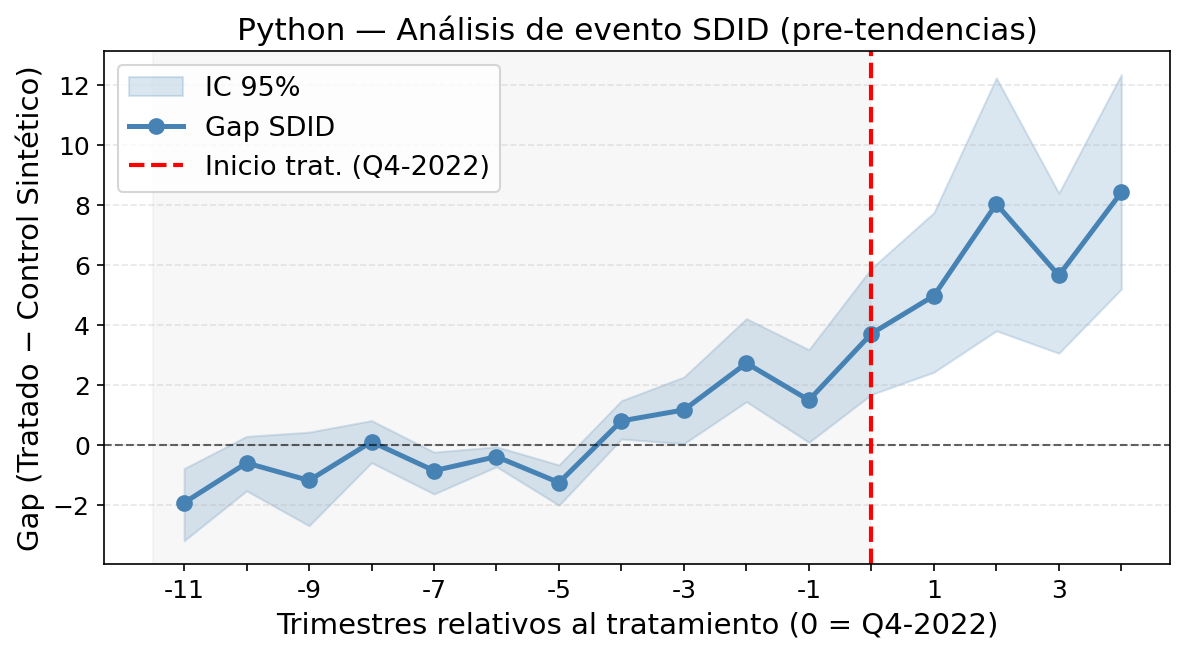
\includegraphics[width=\textwidth,height=0.74\textheight,keepaspectratio]{Pythonsdid_event_study.png}

\vspace{0.1em}
\footnotesize \textbf{Pre-tendencia plana} (gap cerca de cero antes de Q4-2022): el supuesto de paralelismo se cumple para Python $\Rightarrow$ el SDID estima el efecto causal de manera consistente.
\end{frame}

% ── A.4 Event study TypeScript ───────────────────────────────────────────────
\begin{frame}{A.4 Event study SDID --- TypeScript}
\centering
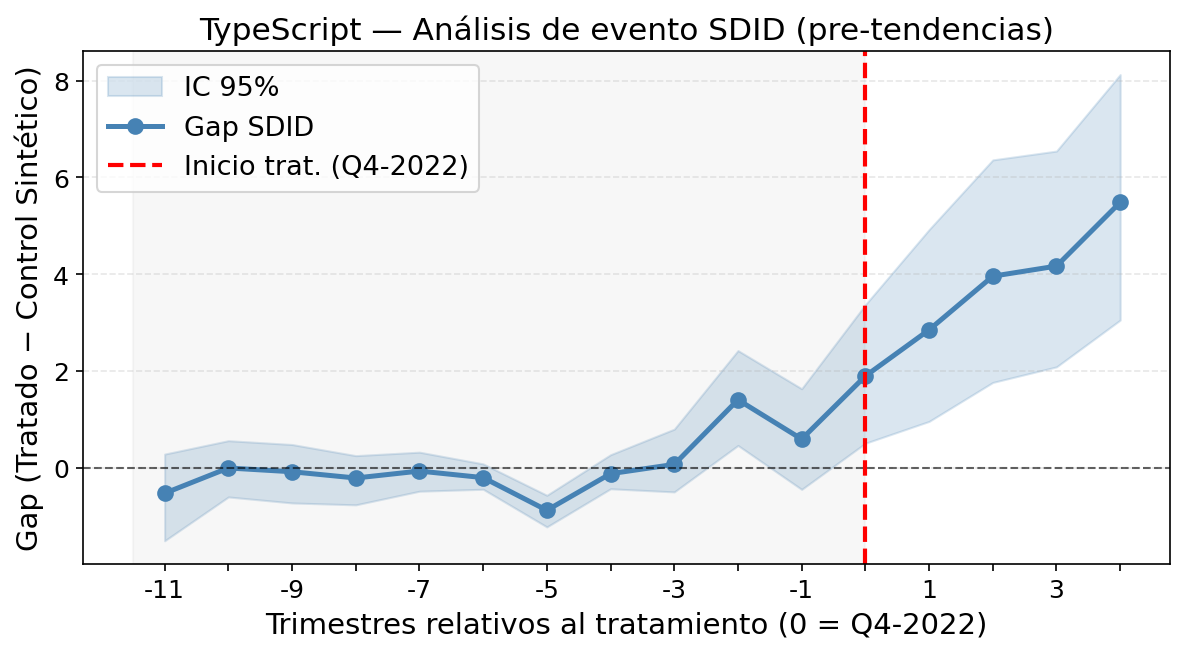
\includegraphics[width=\textwidth,height=0.74\textheight,keepaspectratio]{TypeScriptsdid_event_study.png}

\vspace{0.1em}
\footnotesize \textbf{Pre-tendencia plana} también para TypeScript. El efecto post-tratamiento es claro y la divergencia ocurre a partir de Q4-2022.
\end{frame}

% ── A.5 Event study JavaScript (contraste) ───────────────────────────────────
\begin{frame}{A.5 Event study SDID --- JavaScript (contraste)}
\centering
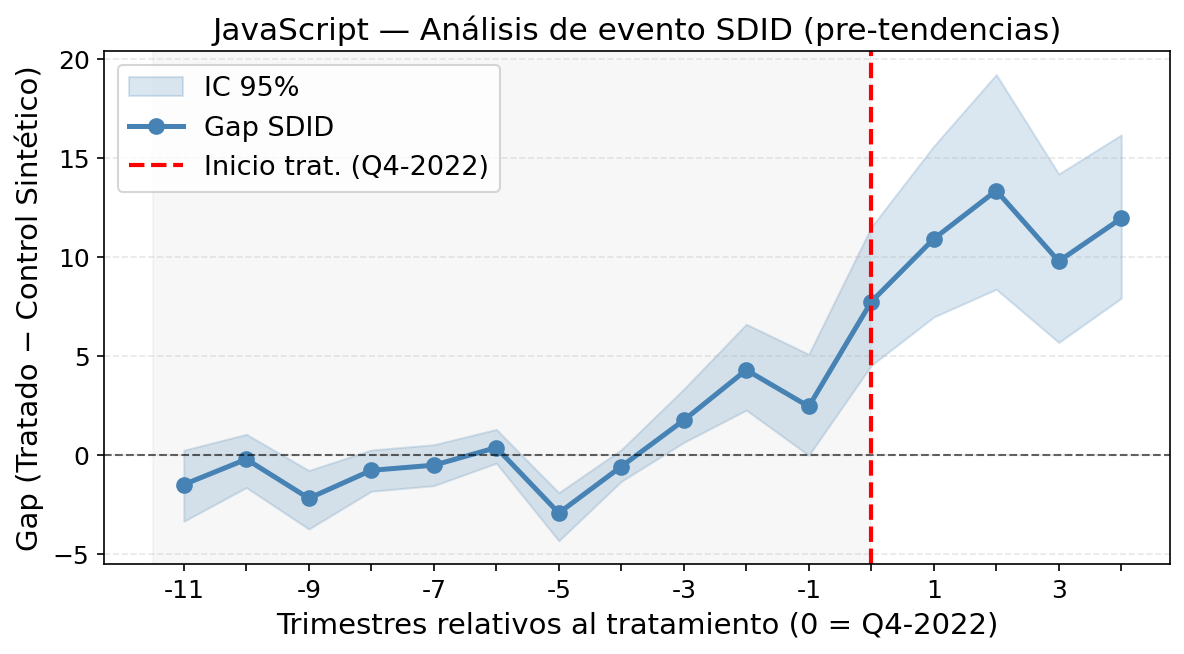
\includegraphics[width=\textwidth,height=0.74\textheight,keepaspectratio]{JavaScriptsdid_event_study.png}

\vspace{0.1em}
\footnotesize \alert{\textbf{Atención:}} en JavaScript se observa una ligera pre-tendencia creciente. El problema es \textbf{específico de este lenguaje}, no del método (ver A.3 y A.4 con pre-tendencias planas).
\end{frame}

% ── A.6 Pesos JavaScript ─────────────────────────────────────────────────────
\begin{frame}{A.6 Pesos del control sintético --- JavaScript}
\centering
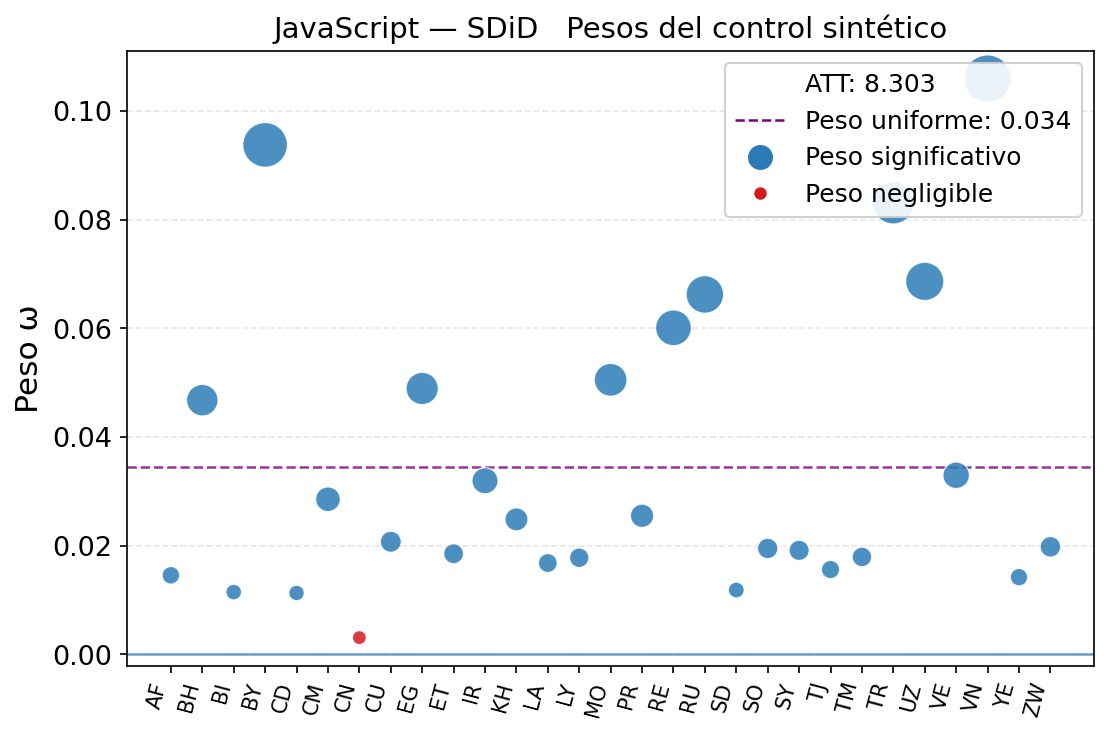
\includegraphics[width=\textwidth,height=0.74\textheight,keepaspectratio]{JavaScriptsdidweights12.png}

\vspace{0.1em}
\footnotesize \textbf{Puntos azules:} donantes con peso significativo ($\geq 30\,\%$ del peso uniforme). El contrafactual de JavaScript se construye con un conjunto diversificado de donantes, lo que reduce dependencia de cualquier país individual.
\end{frame}

% ════════════════════════════════════════════════════════════════════════════
% APÉNDICE B — DERIVACIÓN FORMAL DEL MARCO TEÓRICO (8 PASOS)
% Proceso completo paso a paso. Respaldo para Q&A sobre el modelo.
% ════════════════════════════════════════════════════════════════════════════

{
\setbeamercolor{background canvas}{bg=pucpblue}
\setbeamercolor{normal text}{fg=white}
\setbeamertemplate{headline}{}
\setbeamertemplate{footline}{}
\begin{frame}[plain]
\vfill
\centering
\color{white}
{\Huge\bfseries Apéndice B}\par
\vspace{0.5em}
{\Large Derivación formal del marco teórico --- 8 pasos}\par
\vfill
\footnotesize
\begin{tabular}{rl}
B.1 & Notación básica del modelo \\
B.2 & Función de producción a nivel de tarea (Paso 1) \\
B.3 & Conjunto de tareas automatizables (Paso 2) \\
B.4 & Ahorro relativo por tarea (Paso 3) \\
B.5 & Ganancia individual: partición con/sin IA (Paso 4.1--4.2) \\
B.6 & Ganancia exacta y reescritura (Paso 4.3--4.4) \\
B.7 & Identidad de covarianza (Paso 4.5) \\
B.8 & Normalización de escala (Paso 4.6) \\
B.9 & Decisión de entrada al mercado (Paso 5) \\
B.10 & Agregación a desarrolladores activos (Paso 6) \\
B.11 & Per cápita, absorción y separabilidad (Paso 7) \\
B.12 & Especificación de panel con efectos fijos (Paso 8) \\
B.13 & Resumen paso a paso \\
B.14 & Síntesis de la derivación \\
\end{tabular}
\vfill
\footnotesize\color{white} En \textcolor{orange!80!white}{naranja} se marcan los pasos que dependen de un supuesto no trivial.
\vfill
\end{frame}
}

% ── B.1 Notación ──────────────────────────────────────────────────────────────
\begin{frame}{B.1 Notación básica del modelo}
\small
\centering
\renewcommand{\arraystretch}{1.2}
\begin{tabular}{ll}
\toprule
\textbf{Símbolo} & \textbf{Significado} \\
\midrule
$z\in[0,1]$ & Tarea elemental de programación \\
$h_c(z)>0$ & Productividad humana en la tarea $z$ del lenguaje $c$ \\
$a_c(z)\ge 0$ & Productividad de ChatGPT en la tarea $z$ \\
$\mu_j\in\{0,1\}$ & Acceso del desarrollador $j$ a ChatGPT \\
$y_{jc}(\mu_j)$ & Producción total del desarrollador $j$ en lenguaje $c$ \\
$\mathcal{Z}^{\mathrm{auto}}_c$ & Conjunto de tareas donde ChatGPT supera al humano \\
$\tau_c$ & Fracción de tareas automatizables \\
$\rho_c$ & Ahorro relativo promedio en tareas automatizables \\
$\phi_i$ & Capacidad de absorción tecnológica del país $i$ \\
$A_{it}$ & Disponibilidad de ChatGPT en país $i$, trimestre $t$ \\
$Y_{ict}$ & \textit{Unique pushers} por 100\,mil hab.\ ($i$, $c$, $t$) \\
\bottomrule
\end{tabular}
\end{frame}

% ── B.2 Paso 1 ────────────────────────────────────────────────────────────────
\begin{frame}{B.2 Función de producción a nivel de tarea (Paso 1)}
\small
El desarrollador elige el método más productivo en cada tarea $z\in[0,1]$, y la producción total integra sobre el continuo de tareas:
\[
y_{jc}(z;\mu_j)=\max\{h_c(z),\,\mu_j\,a_c(z)\},
\qquad
y_{jc}(\mu_j)=\int_0^1\max\{h_c(z),\,\mu_j\,a_c(z)\}\,dz.
\]
\begin{itemize}\small
  \item $\mu_j=0$ (sin IA): $\ y_{jc}(0)=\int_0^1 h_c(z)\,dz\ $ (pues $h_c(z)>0$).
  \item $\mu_j=1$ (con IA): $\ y_{jc}(1)=\int_0^1\max\{h_c,a_c\}\,dz\ \ge\ y_{jc}(0)$ puntualmente.
\end{itemize}
\end{frame}

% ── B.3 Paso 2 ────────────────────────────────────────────────────────────────
\begin{frame}{B.3 Conjunto de tareas automatizables (Paso 2)}
\small
Tareas con ganancia marginal estricta de la IA, y reescritura del máximo con la indicadora:
\[
\mathcal{Z}^{\mathrm{auto}}_c=\{z:a_c(z)>h_c(z)\},
\quad
\max\{h_c,a_c\}=h_c\,\mathbf{1}[z\notin\mathcal{Z}^{\mathrm{auto}}_c]+a_c\,\mathbf{1}[z\in\mathcal{Z}^{\mathrm{auto}}_c].
\]
\textbf{Comprobación por casos:}
\begin{itemize}\small
  \item $z\in\mathcal{Z}^{\mathrm{auto}}_c$: $a_c>h_c$, el máx.\ es $a_c$; indicadoras $1$ y $0$. \checkmark
  \item $z\notin\mathcal{Z}^{\mathrm{auto}}_c$: $a_c\le h_c$, el máx.\ es $h_c$; indicadoras $0$ y $1$. \checkmark
\end{itemize}
Medida de tareas automatizables: $\ \tau_c=\int_0^1\mathbf{1}[a_c>h_c]\,dz\in[0,1]$.
\end{frame}

% ── B.4 Paso 3 ────────────────────────────────────────────────────────────────
\begin{frame}{B.4 Ahorro relativo por tarea automatizable (Paso 3)}
\small
Para $z\in\mathcal{Z}^{\mathrm{auto}}_c$, el ahorro relativo que aporta la IA:
\[
s_c(z)=\frac{a_c(z)-h_c(z)}{h_c(z)}>0
\qquad(\text{pues } a_c>h_c>0).
\]
Ahorro promedio \emph{condicional} a las tareas automatizables:
\[
\rho_c=\frac{1}{\tau_c}\int_{\mathcal{Z}^{\mathrm{auto}}_c}s_c(z)\,dz,\qquad \tau_c>0.
\]
\medskip
{\footnotesize\textit{Nota:} si $\tau_c=0$ no hay tareas automatizables y el efecto se interpreta como nulo.}
\end{frame}

% ── B.5 Paso 4.1–4.2 ──────────────────────────────────────────────────────────
\begin{frame}{B.5 Ganancia individual: partición con/sin IA (Paso 4.1--4.2)}
\small
Sustituyendo la reescritura con indicadoras y usando $\int_0^1 f\,\mathbf{1}[z\in A]\,dz=\int_A f\,dz$:
\begin{align*}
\text{Con IA:}\quad y_{jc}(1)&=\int_{[0,1]\setminus\mathcal{Z}^{\mathrm{auto}}_c}\!h_c\,dz+\int_{\mathcal{Z}^{\mathrm{auto}}_c}\!a_c\,dz, \\[2pt]
\text{Sin IA:}\quad y_{jc}(0)&=\int_{[0,1]\setminus\mathcal{Z}^{\mathrm{auto}}_c}\!h_c\,dz+\int_{\mathcal{Z}^{\mathrm{auto}}_c}\!h_c\,dz.
\end{align*}
Ambas comparten exactamente el término sobre las tareas \emph{no} automatizables.
\end{frame}

% ── B.6 Paso 4.3–4.4 ──────────────────────────────────────────────────────────
\begin{frame}{B.6 Ganancia exacta y reescritura (Paso 4.3--4.4)}
\small
Al restar, el término de tareas no automatizables se \textbf{cancela}:
\[
\Delta y_{jc}=y_{jc}(1)-y_{jc}(0)=\int_{\mathcal{Z}^{\mathrm{auto}}_c}\!\bigl[a_c(z)-h_c(z)\bigr]\,dz.
\]
Usando $s_c=\dfrac{a_c-h_c}{h_c}\ \Rightarrow\ a_c-h_c=h_c\,s_c$:
\[
\boxed{\ \Delta y_{jc}=\int_{\mathcal{Z}^{\mathrm{auto}}_c}\!h_c(z)\,s_c(z)\,dz\ }
\]
{\footnotesize\textit{Nota:} hasta aquí todo es \textbf{identidad exacta} --- la derivación no ha impuesto ningún supuesto.}
\end{frame}

% ── B.7 Paso 4.5 ──────────────────────────────────────────────────────────────
\begin{frame}{B.7 Identidad de covarianza (Paso 4.5)}
\small
Definiendo los promedios condicionales sobre $\mathcal{Z}^{\mathrm{auto}}_c$,
$\ \bar h_c=\tfrac{1}{\tau_c}\!\int_{\mathcal{Z}^{\mathrm{auto}}_c}\!h_c\,dz\ $ y $\ \rho_c=\tfrac{1}{\tau_c}\!\int_{\mathcal{Z}^{\mathrm{auto}}_c}\!s_c\,dz$, y aplicando la \textbf{identidad de covarianza}:
\[
\mathbb{E}_{\mathcal{Z}^{\mathrm{auto}}_c}[h_c\,s_c]=\mathbb{E}[h_c]\,\mathbb{E}[s_c]+\mathrm{Cov}(h_c,s_c)
\ \Rightarrow\
\Delta y_{jc}=\tau_c\bigl[\bar h_c\rho_c+\mathrm{Cov}_{\mathcal{Z}^{\mathrm{auto}}_c}(h_c,s_c)\bigr].
\]
\begin{alertblock}{\small Supuesto 1 --- covarianza cero}
\centering Imponer $\mathrm{Cov}(h_c,s_c)=0\ \Rightarrow\ \Delta y_{jc}=\tau_c\,\rho_c\,\bar h_c$.
\end{alertblock}
{\footnotesize\textit{Nota:} es el \textbf{primer} supuesto no trivial; exige que productividad humana $h_c$ y ahorro relativo $s_c$ no estén correlacionados dentro de $\mathcal{Z}^{\mathrm{auto}}_c$.}
\end{frame}

% ── B.8 Paso 4.6 ──────────────────────────────────────────────────────────────
\begin{frame}{B.8 Normalización de escala (Paso 4.6)}
\small
Se elige la unidad de producción tal que el promedio de productividad humana en las tareas automatizables sea unitario, $\bar h_c=1$:
\[
\boxed{\ \Delta y_{jc}=\tau_c\,\rho_c\ }
\]
Es decir, la ganancia individual es el producto \textbf{fracción automatizable} ($\tau_c$) $\times$ \textbf{ahorro relativo promedio} ($\rho_c$), que más adelante define la exposición del lenguaje $\theta_c$.
\medskip
{\footnotesize\textit{Nota:} no es un resultado empírico, es una \textbf{elección de escala}.}
\end{frame}

% ── B.9 Paso 5 ────────────────────────────────────────────────────────────────
\begin{frame}{B.9 Decisión de entrada al mercado (Paso 5)}
\small
Utilidad de programar $U_{\mathrm{prog}}=\eta+y_{jc}(\mu_j)$ frente a la reserva $U_{\mathrm{out}}=r_i$; se entra si $\eta+y_{jc}(\mu_j)\ge r_i$. Umbral mínimo de habilidad:
\[
\eta^*_c(\mu)=r_i-y_{jc}(\mu)\ \Longrightarrow\ \eta^*_c(1)=\eta^*_c(0)-\underbrace{\tau_c\rho_c}_{\Delta y_{jc}}.
\]
El acceso a IA \textbf{reduce} el umbral de habilidad $\Rightarrow$ entran programadores marginales.
\smallskip\\
{\footnotesize\textit{Nota:} con la covarianza exacta, $\ \eta^*_c(1)=\eta^*_c(0)-\tau_c\bigl[\bar h_c\rho_c+\mathrm{Cov}(h_c,s_c)\bigr]$.}
\end{frame}

% ── B.10 Paso 6 ───────────────────────────────────────────────────────────────
\begin{frame}{B.10 Agregación a desarrolladores activos (Paso 6)}
\small
Con población $N_i$ y CDF de habilidad $F_i$ (densidad $f_i$):
\[
\mathrm{Devs}_{ic}(\mu)=N_i\bigl[1-F_i(\eta^*_c(\mu))\bigr].
\]
Taylor de primer orden alrededor de $\eta^*_c(0)$, con $\Delta\eta=\tau_c\rho_c$:
\[
\mathrm{Devs}_{ic}(1)-\mathrm{Devs}_{ic}(0)\approx N_i\,f_i\!\bigl(\eta^*_c(0)\bigr)\,\tau_c\rho_c.
\]
\medskip
{\footnotesize\textit{Nota:} la aproximación de Taylor es válida si $\Delta\eta=\tau_c\rho_c$ es pequeño frente a la escala en que cambia la densidad $f_i$.}
\end{frame}

% ── B.11 Paso 7 ───────────────────────────────────────────────────────────────
\begin{frame}{B.11 Per cápita, absorción y separabilidad (Paso 7)}
\small
Resultado por cada 100\,000 habitantes:
\[
\Delta Y_{ic}=\frac{\mathrm{Devs}_{ic}(1)-\mathrm{Devs}_{ic}(0)}{N_i}\cdot10^5
\approx \underbrace{10^5 f_i(\eta^*_c(0))}_{\phi_i}\cdot\underbrace{\tau_c\rho_c}_{\theta_c}\equiv\phi_i\,\theta_c.
\]
\begin{alertblock}{\small Supuesto 4 --- separabilidad país--lenguaje}
\footnotesize Como $\eta^*_c(0)=r_i-y_{jc}(0)$ depende de $c$, en rigor $\phi_{ic}=10^5 f_i(\eta^*_c(0))$. Escribir $\phi_i$ (solo país) exige $f_i(\eta^*_c(0))\approx f_i$ (densidad plana en $c$), o equivalentemente que las productividades base $y_{jc}(0)$ sean similares entre lenguajes.
\end{alertblock}
{\footnotesize\textit{Nota:} sin separabilidad el ATT por lenguaje sigue identificado, pero como $\theta_c\,\bar\phi_{\mathcal{T},c}$ (absorción promedio del lenguaje).}
\end{frame}

% ── B.12 Paso 8 ───────────────────────────────────────────────────────────────
\begin{frame}{B.12 Especificación de panel con efectos fijos (Paso 8)}
\small
Descomponiendo la línea base $Y_{ic}(0)=\alpha_i+\beta_t+\delta_c+\eta_{ict}$ y sustituyendo $\Delta Y_{ic}\approx\theta_c\phi_i\,A_{it}$ (con $A_{it}\in\{0,1\}$):
\[
\boxed{\ Y_{ict}=\alpha_i+\beta_t+\delta_c+\theta_c\,\phi_i\,A_{it}+\eta_{ict}\ }
\]
Para interpretación \emph{causal} se requiere exogeneidad condicional:
\[
\mathbb{E}[\eta_{ict}\mid\alpha_i,\beta_t,\delta_c,A_{it}]=0.
\]
\end{frame}

% ── B.13 Resumen ──────────────────────────────────────────────────────────────
\begin{frame}{B.13 Resumen paso a paso}
\scriptsize
\renewcommand{\arraystretch}{1.25}
\centering
\begin{tabular}{>{\bfseries}c p{6.0cm} p{4.7cm}}
\toprule
Paso & \textbf{Resultado} & \textbf{Tipo} \\
\midrule
1 & $y_{jc}(\mu_j)=\int_0^1\max\{h_c,\mu_j a_c\}dz$ & Identidad / definición \\
2 & $\tau_c=\int_0^1\mathbf{1}[a_c>h_c]\,dz$ & Definición exacta \\
3 & $\rho_c=\frac{1}{\tau_c}\int s_c\,dz$ & Definición exacta ($\tau_c>0$) \\
4.1--4.4 & $\Delta y_{jc}=\int_{\mathcal{Z}^{\mathrm{auto}}_c}h_c s_c\,dz$ & Identidad exacta \\
4.5 & $\Delta y_{jc}=\tau_c\rho_c\bar h_c$ & \textcolor{naranjasupp}{\textbf{Supuesto}: $\mathrm{Cov}(h_c,s_c)=0$} \\
4.6 & $\Delta y_{jc}=\tau_c\rho_c$ & Normalización $\bar h_c=1$ \\
5 & $\eta^*_c(1)=\eta^*_c(0)-\tau_c\rho_c$ & Depende del Paso 4 \\
6 & $\approx N_i f_i(\eta^*_c(0))\,\tau_c\rho_c$ & Taylor 1.\textordmasculine\ orden \\
7 & $\Delta Y_{ic}\approx\theta_c\phi_i$ & \textcolor{naranjasupp}{Aprox.\ + separabilidad $\phi_{ic}\!\approx\!\phi_i$} \\
8 & $Y_{ict}=\alpha_i+\beta_t+\delta_c+\theta_c\phi_i A_{it}+\eta_{ict}$ & Especificación de panel \\
\bottomrule
\end{tabular}

\vspace{0.5em}
\footnotesize En \textcolor{naranjasupp}{naranja}, los pasos que dependen de un \textbf{supuesto no trivial}; el resto son identidades o definiciones exactas.
\end{frame}

% ── B.14 Conclusión ───────────────────────────────────────────────────────────
\begin{frame}{B.14 Síntesis de la derivación}
\small
La construcción no requiere ningún supuesto hasta $\ \Delta y_{jc}=\int_{\mathcal{Z}^{\mathrm{auto}}_c}h_c(z)\,s_c(z)\,dz$. De aquí en adelante se introducen los supuestos del modelo. La forma general de la ganancia individual es:
\[
\Delta y_{jc}=\tau_c\bigl[\bar h_c\,\rho_c+\mathrm{Cov}_{\mathcal{Z}^{\mathrm{auto}}_c}(h_c,s_c)\bigr],
\]
de la cual $\tau_c\rho_c\bar h_c$ es el caso particular con covarianza nula. La ecuación estimable $Y_{ict}=\alpha_i+\beta_t+\delta_c+\theta_c\phi_i A_{it}+\eta_{ict}$ se obtiene como modelo estructural simplificado a partir de \textbf{cuatro} supuestos:
\begin{enumerate}\footnotesize
  \item \textbf{Covarianza cero} entre productividad humana $h_c(z)$ y ahorro relativo $s_c(z)$ dentro de $\mathcal{Z}^{\mathrm{auto}}_c$.
  \item \textbf{Normalización} $\bar h_c=1$ (elección de escala).
  \item \textbf{Taylor de 1.\textordmasculine\ orden} para pasar de la caída del umbral al aumento de desarrolladores.
  \item \textbf{Separabilidad país--lenguaje} ($\phi_{ic}\approx\phi_i$) para factorizar el coeficiente como $\theta_c\phi_i$.
\end{enumerate}
\end{frame}

\end{document}
